\documentclass[final,onefignum,onetabnum]{siamart220329}

%% ------------------------------------------------------------------
%% Code used in examples, needed to reproduce 
%% ------------------------------------------------------------------
%% Used for \set, used in an example bow
\usepackage{braket,amsfonts}

%% Used in table example below
\usepackage{array}

%% Used in table and figure examples below
\usepackage[caption=false]{subfig}
%% Used for papers with subtables created with the subfig package
\captionsetup[subtable]{position=bottom}
\captionsetup[table]{position=bottom}

%% Used for PgfPlots example, shown in the "Figures" section below.
\usepackage{pgfplots}

%% Used for creating new theorem and remark environments
\newsiamthm{claim}{Claim}
\newsiamremark{remark}{Remark}
\newsiamremark{hypothesis}{Hypothesis}
\crefname{hypothesis}{Hypothesis}{Hypotheses}

%% Algorithm style, could alternatively use algpseudocode
\usepackage{algorithmic}

%% For figures
\usepackage{graphicx,epstopdf}

%% For referencing line numbers
\Crefname{ALC@unique}{Line}{Lines}

%% For creating math operators
\usepackage{amsopn}
\DeclareMathOperator{\Range}{Range}

% Custom
\usepackage[utf8]{inputenc}
\usepackage[english]{babel}
\usepackage{siunitx}
\usepackage{hyperref}
% Math packages
\usepackage{amsmath}
\usepackage{amsfonts}
\usepackage{amssymb}

\let\oldhat\hat
\renewcommand{\hat}[1]{\mathbf{\oldhat{#1}}}

\newcommand{\bn}{\bold{n}}
\newcommand{\bx}{\boldsymbol{x}}
\newcommand{\bhx}{{\bold{\hat{x}}}}
\newcommand{\bhy}{\bold{\hat{y}}}
\newcommand{\hx}{{\hat{x}}}
\newcommand{\hy}{{\hat{y}}}
\newcommand{\hvarphi}{{\hat{\varphi}}}
\newcommand{\hPhi}{{\hat{\Phi}}}
\newcommand{\by}{\boldsymbol{y}}
\newcommand{\br}{\boldsymbol{r}}
\newcommand{\btheta}{\bold{\theta}}
\newcommand{\htau}{{\hat{\tau}}}
\newcommand{\hpsi}{{\hat{\psi}}}
\newcommand{\M}{\mathcal{T}}
\newcommand{\tensor}[1]{\overline{\overline{\boldsymbol{#1}}}}
\newcommand{\chia}{\chi^{\text{affine}}}
\newcommand{\pt}{\bold{P}}
\newcommand{\uapprox}{u^{\text{approx}}}
\newcommand{\uref}{u^{\text{ref}}}

\newcommand{\bol}{\boldsymbol}
\newcommand{\nee}{\bold{e}}
\newcommand{\nej}{\bold{j}}
\newcommand{\nem}{\bold{m}}
\newcommand{\nephi}{\boldsymbol{\phi}}
\newcommand{\nepsi}{\boldsymbol{\psi}}
\newcommand{\new}{\boldsymbol w}
\newcommand{\ney}{\boldsymbol{y}}
\newcommand{\nex}{\boldsymbol{x}}
\newcommand{\bnex}{\bold{x}}
\newcommand{\nez}{\boldsymbol{z}}
\newcommand{\nev}{\boldsymbol{v}}
\newcommand{\neu}{\boldsymbol{u}}
\newcommand{\nerho}{\boldsymbol{\varrho}}
\newcommand{\ner}{\bol{r}}
\newcommand{\TE}{\mathrm{TE}}
\newcommand{\TM}{\mathrm{TM}}
\newcommand{\de}{\,\mathrm{d}}
\newcommand{\e}{\operatorname{e}}
\newcommand{\im}{\operatorname{i}}
\newcommand{\inc}{\mathrm{inc}}
\newcommand{\rad}{\mathrm{rad}}
\newcommand{\gui}{\mathrm{gui}}
\newcommand{\ontext}{\quad\mbox{on}\quad}
\newcommand{\intext}{\quad\mbox{in}\quad}
\newcommand{\andtext}{\quad\mbox{and}\quad}
\newcommand{\dtn}{\mathcal{B}}
\newcommand{\dtnn}{\mathrm{T}}
\newcommand{\sovo}{\operatorname{H}}
\newcommand{\keps}{k_{\varepsilon}}
\newcommand{\p}{\partial}
\newcommand{\cp}{\times}
\newcommand{\mpt}{\mathbf A}
\newcommand{\crt}{\mathbf J}
\newcommand{\dygfn}{\bar{\bold G}}
\newcommand{\untx}{\hat x}
\newcommand{\unty}{\hat y}
\newcommand{\untz}{\hat z}
\newcommand{\teps}{\boldsymbol{\overline\epsilon}}
\newcommand{\tmu}{\boldsymbol{\overline\mu}}
\newcommand{\ftr}{\widehat{F}}
\newcommand{\dlpfs}{\bold{K}^{\mathrm{fs}}}
\newcommand{\dlphs}{\bold{K}^{\mathrm{hs}}}
\newcommand{\slpfs}{\bold{S}^{\mathrm{fs}}}
\newcommand{\slphs}{\bold{S}^{\mathrm{hs}}}
\newcommand{\real}{\mathrm{Re}\,}
\newcommand{\uinc}{u_{\mathrm{inc}}}
\newcommand{\imag}{\mathrm{Im}\,}
\newcommand{\inte}{\mathrm{int}}
\newcommand{\exte}{\mathrm{ext}}
\newcommand{\lf}{\left}
\newcommand{\rg}{\right}
\newcommand{\tdir}{\widehat{\boldsymbol \theta}}
\newcommand{\rdir}{\widehat{\boldsymbol r}}
\newcommand{\xdir}{\widehat{\bold i}}
\newcommand{\ydir}{\widehat{\bold j}}
\newcommand{\zdir}{\widehat{\bold k}}
\newcommand{\R}{\mathbb{R}}
\newcommand{\C}{\mathbb{C}}
\newcommand{\N}{\mathbb{N}}
\newcommand{\elc}{\mathbf E}
\newcommand{\mgn}{\mathbf H}
\newcommand{\mgf}{\bold H}
\newcommand{\elf}{\bold E}
\newcommand{\can}{\bold e}
\newcommand{\normal}{n}
\newcommand{\nor}{\bold n}
\newcommand{\curl}{\operatorname{curl}}
\newcommand{\grd}{\operatorname{grad}}
\newcommand{\dv}{\operatorname{div}}
\newcommand{\vecphi}{\boldsymbol{\upphi}}

\newcommand{\Dcal}{\mathcal{D}}
\newcommand{\Gcal}{\mathcal{G}}
\newcommand{\Hcal}{\mathcal{H}}
\newcommand{\Ical}{\mathcal{I}}
\newcommand{\Lcal}{\mathcal{L}}
\newcommand{\Mcal}{\mathcal{M}}
\newcommand{\Ocal}{\mathcal{O}}
\newcommand{\Pcal}{\mathcal{P}}
\newcommand{\Qcal}{\mathcal{Q}}
\newcommand{\Scal}{\mathcal{S}}
\newcommand{\Wcal}{\mathcal{W}}
\newcommand{\Tcal}{\mathcal{T}}
\newcommand{\Kcal}{\mathcal{K}}
\newcommand{\tG}{\mathbb{G}}
\newcommand{\tId}{\mathbb{I}}
\newcommand{\Tbf}{\mathbf{T}}

\newcommand{\bigo}[1]{\Ocal\left(#1\right)}
\newcommand{\abs}[1]{\left|#1\right|}
\newcommand{\norm}[1]{\left\|#1\right\|}

%% ------------------------------------------------------------------
%% Macros for in-document examples. These are not meant to reused for
%% SIAM journal papers.
%% ------------------------------------------------------------------
\usepackage{xspace}
\usepackage{bold-extra}
\usepackage[most]{tcolorbox}
\newcommand{\BibTeX}{{\scshape Bib}\TeX\xspace}
\newcounter{example}
\colorlet{texcscolor}{blue!50!black}
\colorlet{texemcolor}{red!70!black}
\colorlet{texpreamble}{red!70!black}
\colorlet{codebackground}{black!25!white!25}

\newcommand\bs{\symbol{'134}} % print backslash in typewriter OT1/T1
\newcommand{\preamble}[2][\small]{\textcolor{texpreamble}{#1\texttt{#2 \emph{\% <- Preamble}}}}

\lstdefinestyle{siamlatex}{%
  style=tcblatex,
  texcsstyle=*\color{texcscolor},
  texcsstyle=[2]\color{texemcolor},
  keywordstyle=[2]\color{texemcolor},
  moretexcs={cref,Cref,maketitle,mathcal,text,headers,email,url},
}

\tcbset{%
  colframe=black!75!white!75,
  coltitle=white,
  colback=codebackground, % bottom/left side
  colbacklower=white, % top/right side
  fonttitle=\bfseries,
  arc=0pt,outer arc=0pt,
  top=1pt,bottom=1pt,left=1mm,right=1mm,middle=1mm,boxsep=1mm,
  leftrule=0.3mm,rightrule=0.3mm,toprule=0.3mm,bottomrule=0.3mm,
  listing options={style=siamlatex}
}

\newtcblisting[use counter=example]{example}[2][]{%
  title={Example~\thetcbcounter: #2},#1}

\newtcbinputlisting[use counter=example]{\examplefile}[3][]{%
  title={Example~\thetcbcounter: #2},listing file={#3},#1}

\DeclareTotalTCBox{\code}{ v O{} }
{ %fontupper=\ttfamily\color{texemcolor},
  fontupper=\ttfamily\color{black},
  nobeforeafter,
  tcbox raise base,
  colback=codebackground,colframe=white,
  top=0pt,bottom=0pt,left=0mm,right=0mm,
  leftrule=0pt,rightrule=0pt,toprule=0mm,bottomrule=0mm,
  boxsep=0.5mm,
  #2}{#1}

% Stretch the pages
\patchcmd\newpage{\vfil}{}{}{}
\flushbottom

\title{An implementation of Neural Ordinary Differential Equations}

\author{Rodrigo Arrieta\thanks{Mathematics Department, Massachusetts Institute of Technology, Cambridge, MA 02139, United States (\email{rarrieta@mit.edu}).}}

\begin{document}
\maketitle

\section{Introduction}
In this report a review of Neural Ordinary Differential Equations (Neural ODEs), as well as an implementation coded in Julia, is presented. Neural ODEs are a class of models that combine neural networks with ordinary differential equations (ODEs). They were introduced by Chen et al. in 2018 \cite{chen2018neural} as a way to learn continuous-time dynamics directly from data.

Unlike traditional approaches, e.g. recurrent neural networks, where data is modeled through a discrete sequence of compositions and transformations, in Neural ODEs data is modeled continuously. In this case, a neural network is used to model the derivative of the data $\bol u:\R\rightarrow\R^N$, which is assumed to be differentiable and continuously dependent on time:
\begin{align}
	\frac{d}{dt}\bol{u}(t) = \text{NN}(\bol{u}(t),t,\bol \theta),
\end{align}
where $\text{NN}$ correspond to a neural network, $t$ is the time variable and $\bol \theta\in \R^M$ are the neural network weights. Then, given an initial condition $\bol u_0 \equiv \bol u(t_0)\in\R^N$, the model prediction at time $t_1$ is obtained through any standard ODE solver, this is
\begin{align}
	\bol{u}(t_1) &= \bol{u}_0 + \int_{t_0}^{t_1} \text{NN}(\bol{u}(t),t,\bol \theta) \de{t}\\
	&= \text{ODESolver}(\text{NN},\bol{u}_0,t_0,t_1). \label{eq:odesolver}
\end{align}

A key advantage of Neural ODEs is their ability to model continuous-time dynamics, making them suitable for tasks where time plays a crucial role, such as time series forecasting, trajectory prediction and generative modeling. By learning the system's latent dynamics, Neural ODEs can capture complex temporal dependencies and generalize well to unseen time points.

Neural ODEs have shown promising results in various domains, including computer vision, natural language processing, and physics, financial and biological simulations \cite{kidger2022neural}. They provide a flexible framework for modeling continuous-time dynamics using neural networks, enabling a deeper understanding of temporal phenomena and latent dynamics in data.

This report is organized as follow. Section \ref{sec:back} explains how backpropagation is performed in Neural ODEs. Sec. \ref{sec:imple} presents our in-house implementation of Neural ODE adjoint solver, coded in Julia from scratch and built on top of the Flux.jl library, alongside with some examples of interests. Finally, Sec. \ref{sec:hnn} presents Hamiltonian Neural Networks, a special case of Neural ODEs specially designed to deal with Hamiltonian systems. Our code and examples can be found in here\footnote{\url{https://github.com/Riarrieta/NeuralODEProject}}.

\section{Backpropagation of Neural ODEs}\label{sec:back}
Training Neural ODEs involves solving an optimization problem to find the parameters that minimize a given loss function, which can be done using gradient-based methods. In the context of Neural ODEs, to obtain the gradient of the loss function, a process called \textit{backpropagation}, which is typically achieved through automatic differentiation in a typical neural network setting, is seldom performed. This is because backpropagating through the forward pass of the ODE solver (eq. \ref{eq:odesolver}) could be prohibitively expensive. Another reason is due to the potential limitation of the automatic differentiation engine's access to an external-library ODE solver. Instead, gradients are obtained through an adjoint sensitivity method, originally presented in \cite{chen2018neural}. This method is explained below.

Suppose the initial condition $\bol u_0$ is given and our loss function $G$ has the form of an integral of our model prediction $\bol u$ in some interval $[0,T]$, i.e.
\begin{align}
	G(\bol{u},\bol\theta) &= \int_0^T g(\bol{u}(t,\bol\theta))\, \de{t}, \label{eq:loss}
\end{align}
where we have made explicit the dependence of the weights $\bol \theta$ in $\bol u$. In a typical setting, we have access to a discrete set of observations $\{\tilde{\bol{u}}(t_i)\}_{i=1}^P$, with $t_i \in [0,T]$, and we wish to minimize the discrete $L^2$ error loss, or mean squared error, given by
\begin{align}
	G(\bol{u},\bol\theta) = \frac{1}{P}\sum_{i=1}^{P}\norm{\tilde{\bol{u}}(t_i)-{\bol{u}}(t_i,\bol \theta)}^2, \label{eq:mse}
\end{align}
in which case
\begin{align}
	g(\bol{u}(t,\bol\theta)) = \frac{1}{P}\sum_{i=1}^{P}\norm{\tilde{\bol{u}}(t_i)-{\bol{u}}(t,\bol \theta)}^2\delta(t-t_i),
\end{align}
where $\delta$ correspond to the Dirac delta function.

The goal of backpropagation is to obtain the gradient $\partial G(\bol{u},\bol\theta) / \partial\bol\theta \in \R^M$ and use it to update the weights of our neural network. To do this we resort to the adjoint method, which consists in the following steps:\\
\begin{enumerate}
	\item \textbf{Forward pass.} Solve for $\bol u$ in the interval $[0,T]$ using the ODE solver (eq. \ref{eq:odesolver}) and evaluate the loss function \eqref{eq:loss}.
	
	\item \textbf{Backward pass.} Define the adjoint variables $\bol\lambda:[0,T] \rightarrow \R^N$ and $\bol\mu:[0,T] \rightarrow \R^M$. They are solutions of the adjoint ODE
	\begin{subequations}
	\begin{align}
		\frac{d}{dt} \bol{\lambda}(t) &= -\left[\frac{\partial }{\partial\bol{u}}\textit{NN}(\bol{u}(t),t,\bol \theta)\right]^\top \bol{\lambda}(t)- \frac{d}{d\bol{u}} g(\bol u (t)),\\
		\frac{d}{dt} \bol{\mu}(t) &= -\left[\frac{\partial }{\partial\bol\theta}\textit{NN}(\bol{u}(t),t,\bol \theta)\right]^\top  \bol{\lambda}(t),\\
		\bol\lambda(T^+) &= \bol 0,\\
		\bol\mu(T^+) &= \bol 0.
	\end{align}\label{eq:adjointode}
	\end{subequations}
	Solve the adjoint ODE backwards in time, from $T^+$ to $0^-$. Note the terms $\tfrac{\partial }{\partial\bol{u}}\textit{NN}^\top \bol{\lambda}$ and $\tfrac{\partial}{\partial\bol{\theta}}\textit{NN}^\top \bol{\lambda}$ can be efficiently evaluated using reverse-mode automatic differentiation and vector-Jacobian products.
	
	\item \textbf{Evaluate gradient.} The gradient of the loss function with respect to the parameters is given by
	\begin{align}
		\frac{\partial}{\partial\bol\theta} G(\bol{u},\bol\theta) = \bol\mu(0^-).
	\end{align}
	
	\item \textbf{Update weights.} Finally, update the neural network weights using the previously obtained gradient.\\
\end{enumerate}

Note that the backward pass requires the values of $\bol u(t)$ for $t\in [0,T]$ in order to solve the adjoint ODE \eqref{eq:adjointode}. Therefore, it is necessary to either (A) store values of $\bol u$ in the forward pass and then use an interpolant of $\bol u$ during the backward pass, or (B) solve for $\bol u$ backward in time during the backward pass. Clearly, method (A) is more memory intensive, whereas method (B) is more compute intensive. Nevertheless, for method (B) it is important to mention that, although ODEs are theoretically reversible in time, it is possible that solving for $\bol u$ backward in time yields a different solution compared to the forward pass, due to the ODE solver discretization errors, thus resulting in an incorrect backward pass solution. For this reason, we have chosen method (A) for our in-house implementation of the Neural ODE adjoint solver (see Sec. \ref{sec:imple}). 

\section{An in-house implementation of a Neural ODE adjoint solver} \label{sec:imple}
In this section we present an in-house implementation of a Neural ODE adjoint solver. It is written in Julia and built on top of the machine learning library Flux.jl \cite{Flux.jl-2018}, the reverse-mode automatic differentiation library Zygote.jl \cite{Zygote.jl-2018} and the ODE solver library OrdinaryDiffEq.jl \cite{DifferentialEquations.jl-2017}. There are already existing packages that implement Neural ODE adjoint solvers, e.g. DiffEqFlux.jl \cite{DiffEqFlux.jl}, but we have decided to implement an adjoint solver from scratch for pedagogical purposes, not only to learn about Neural ODEs, but also with the purpose of us getting acquainted with the Flux.jl library. Our code and examples can be found in here\footnote{\url{https://github.com/Riarrieta/NeuralODEProject}}.

In the following subsections, we will showcase some examples of interest conducted using our code. In all of these examples, we employed a neural network with a single hidden layer consisting of 64 hidden units, \textit{tanh} activation functions, and a loss function given by the mean square error \eqref{eq:mse}. We used the ODE solver \textit{tsit5} of the OrdinaryDiffEq.jl package. 

\subsection{Example: linear system}\label{ex:linear}
Consider the linear constant-coefficient ODE 
\begin{align}
	\frac{d}{dt}\bol{u}(t) = A\bol{u}(t) 
\end{align}
in the interval $[0,1]$, with
\begin{align}
	A &= \begin{pmatrix}
		-0.1 & 2 \\
		-2 & -0.1
	\end{pmatrix}.
\end{align}
We trained our neural network with 11 uniformly spaced observation in $[0,1]$ for various normal random initial conditions $\bol u_0 \sim \mathcal{N}(\mu=0,\sigma=4)$. A comparison between the true solution, for a random initial condition, and our Neural ODE solution is shown in Fig. \ref{fig:linear_comparison}. We observe that after enough training our Neural ODE solution is able to follow the true solution quite well inside the training interval. Furthermore, if we extend the ODE and Neural ODE solution outside the training interval, as shown in Fig. \ref{fig:linear_extrapolation}, the Neural ODE keeps up with the true solution if we go forward in time, where the amplitude of the true solution decreases. Nevertheless, if we go backward in time, the amplitude of the true solution increases and the Neural ODE is not able to follow. This in an expected behavior. For large amplitudes the nonlinear activation functions start to kick in, removing the neural network from its linear behavior, thus the (nonlinear) Neural ODE cannot keep up with the true linear ODE. Clearly, this issue can be overcome by training the neural network with initial conditions of larger and larger amplitude, however, for a fixed neural network, a sufficiently large amplitude will remove it from its linear behavior. This simple example illustrates the limitation of using Neural ODEs to model ODEs with unbounded solutions over time.

\begin{figure}[h!]
	\centering
	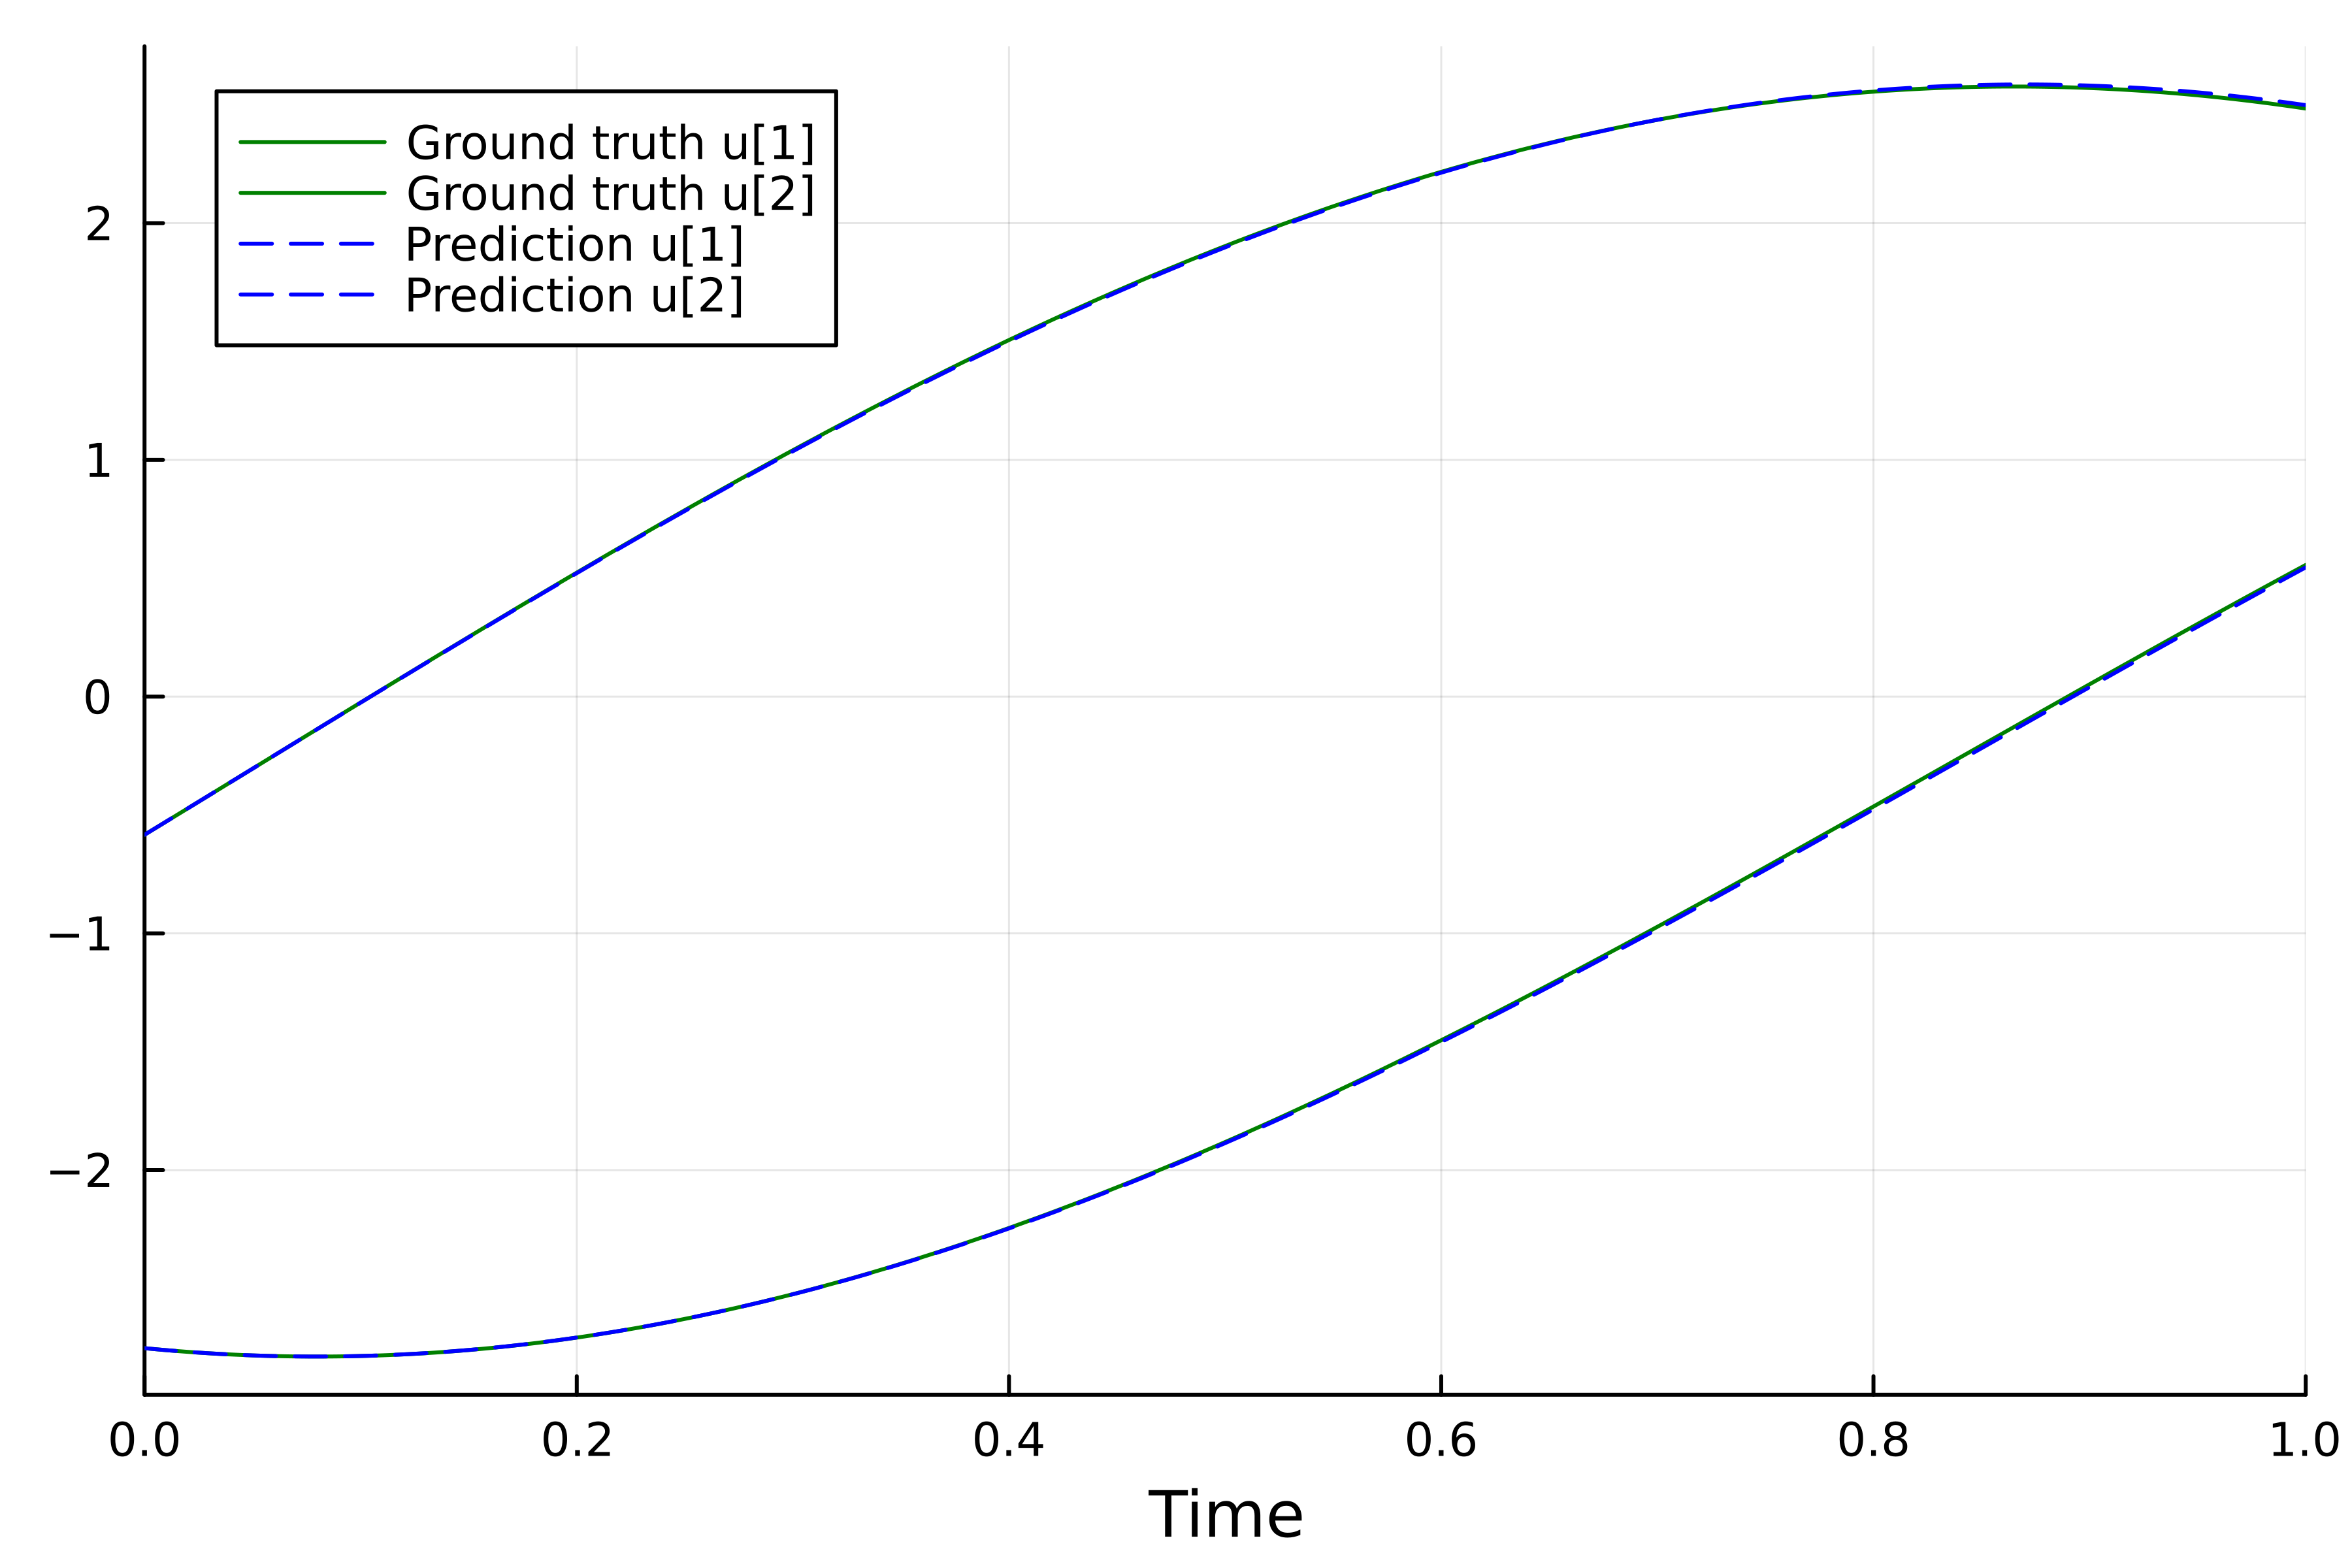
\includegraphics[width=0.5\linewidth]{../examples/linear/comparison}
	\caption{Example \ref{ex:linear}. Comparison between the true solution and our Neural ODE solution in the training interval $[0,1]$.}
	\label{fig:linear_comparison}
\end{figure}

\begin{figure}[h!]
	\centering
	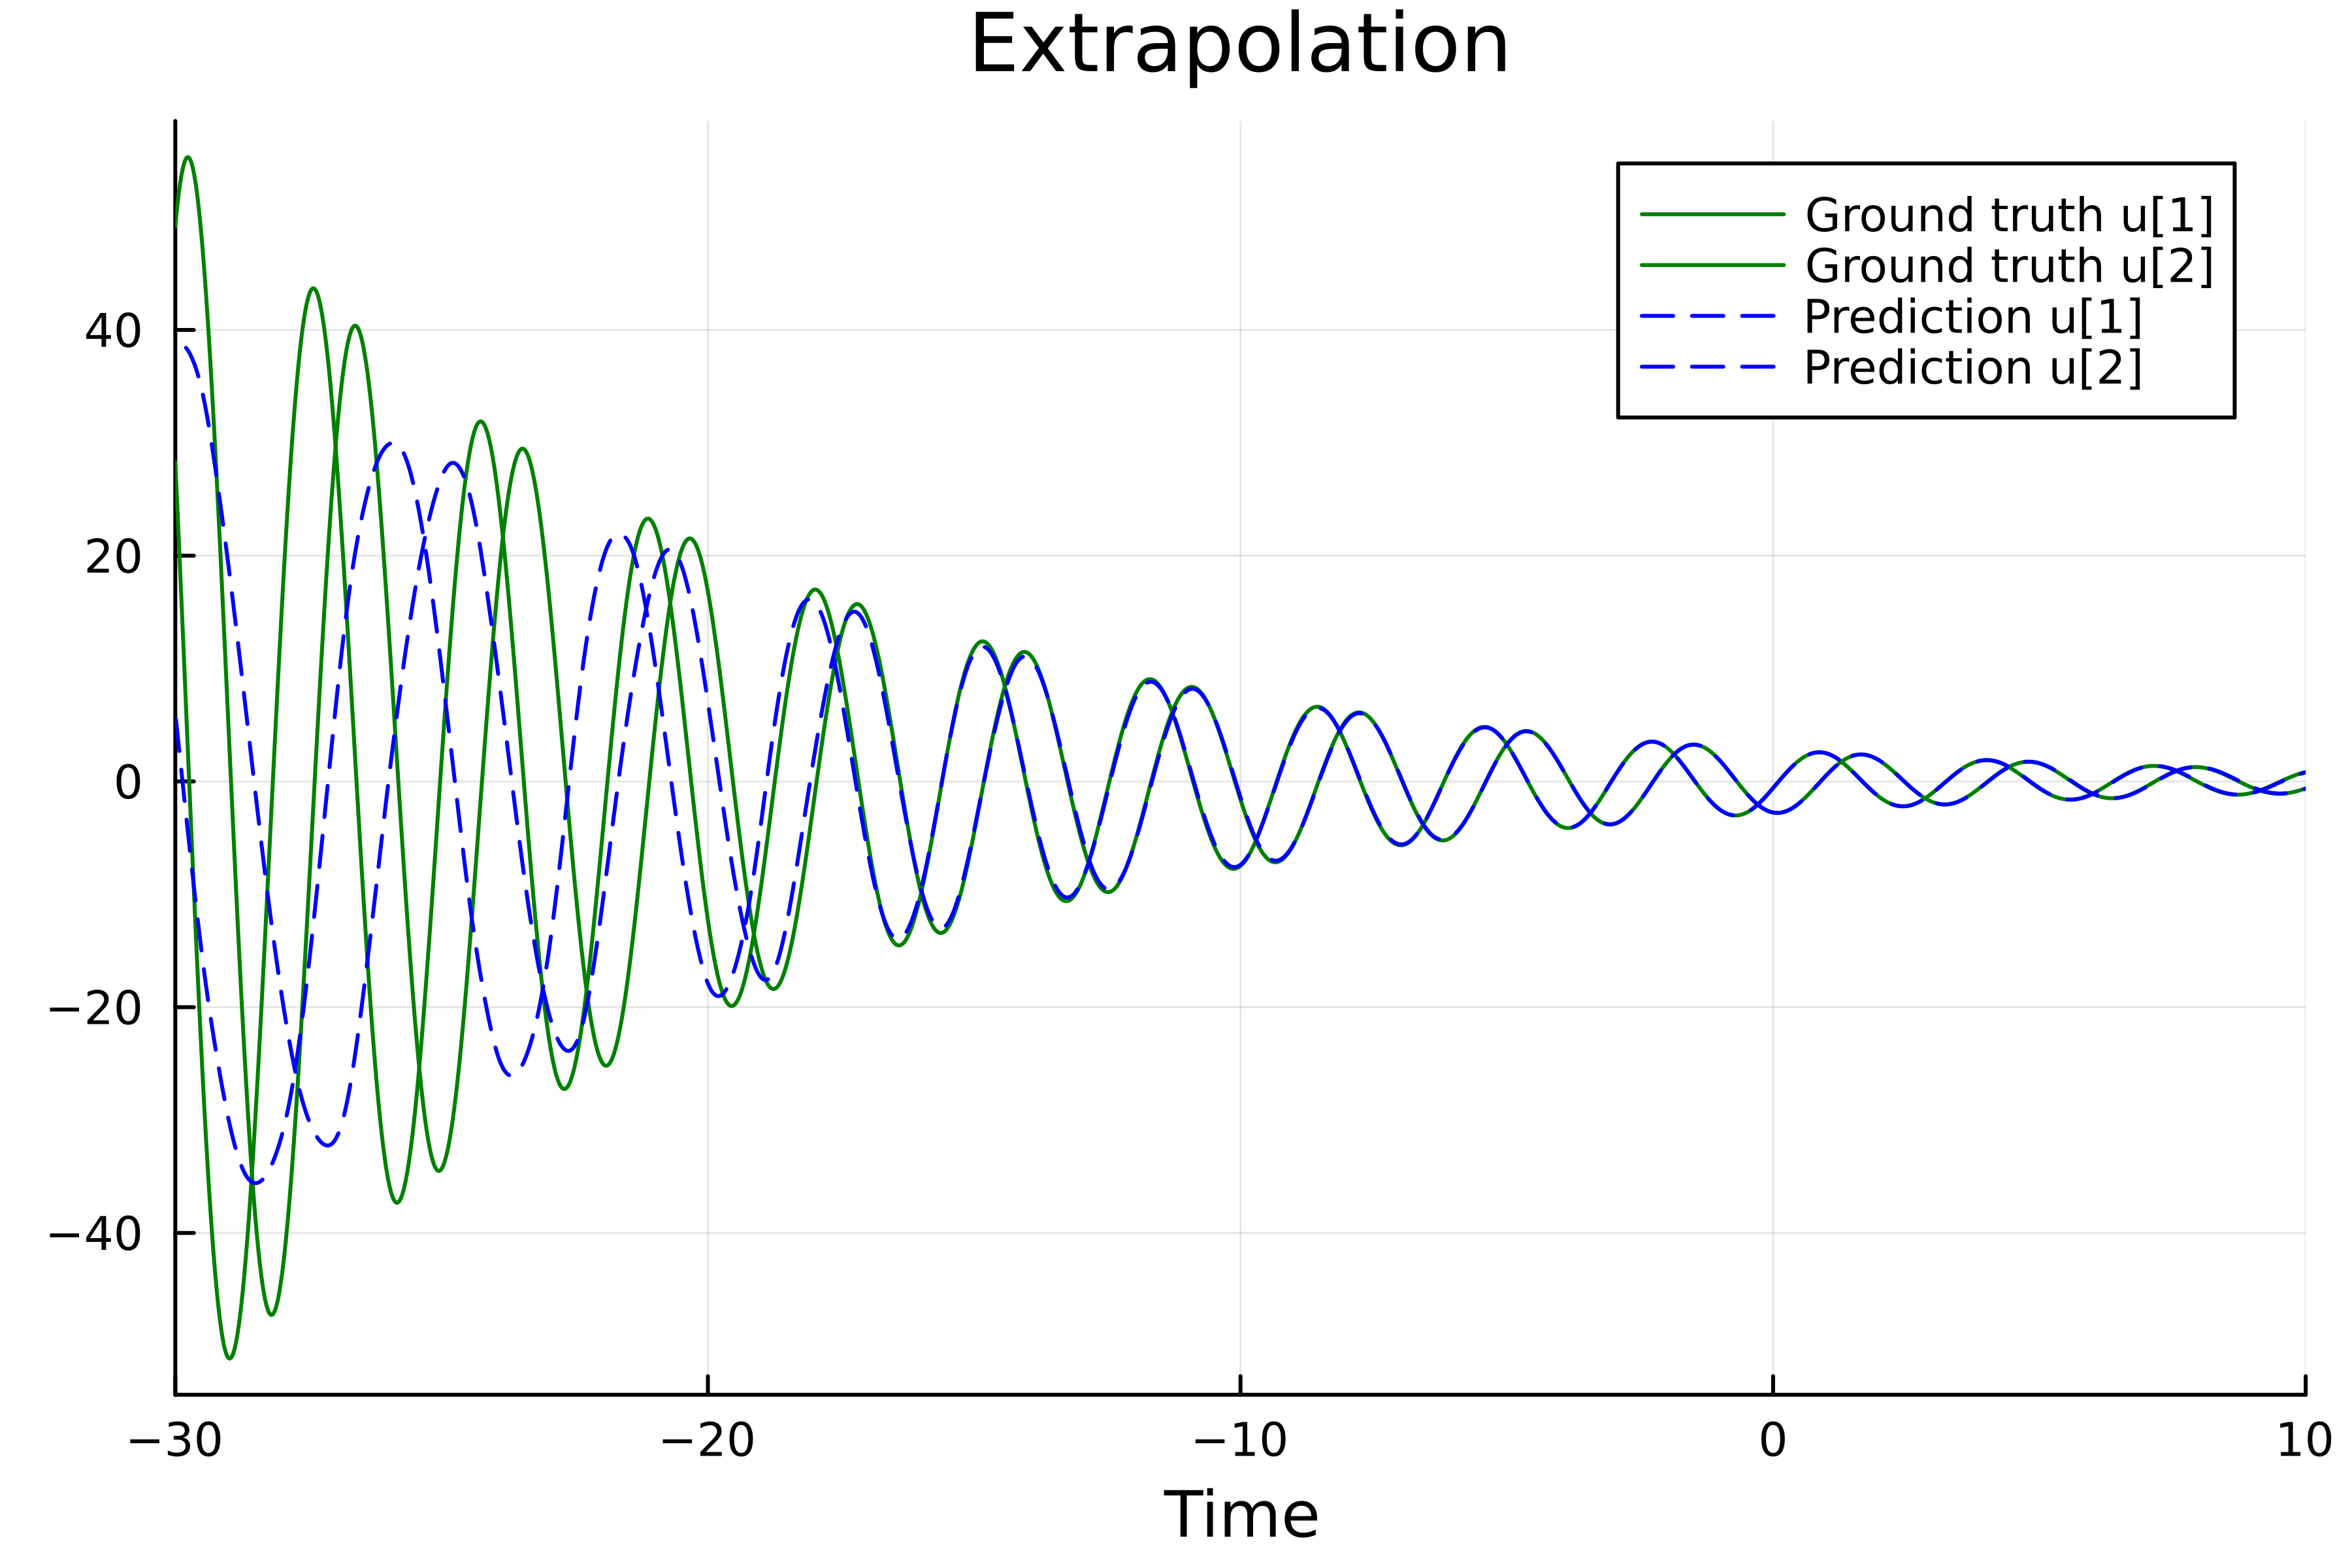
\includegraphics[width=0.5\linewidth]{../examples/linear/extrapolation}
	\caption{Example \ref{ex:linear}. Extrapolation of the ODE and Neural ODE solution outside the training interval.}
	\label{fig:linear_extrapolation}
\end{figure}

\subsection{Example: Lotka-Volterra equations}\label{ex:lotka_volterra}
Consider the Lotka-Volterra equations
\begin{align}
	\frac{d}{dt}x(t) &= \alpha x(t) - \beta x(t) y(t),\\
	\frac{d}{dt}y(t) &= \delta x(t)y(t) - \gamma y(t),
\end{align}
in the interval $[0,10]$ with parameters $(\alpha, \beta, \delta, \gamma) = (2/3, 4/3, 1, 1)$ and initial condition $(x_0,y_0) = (1,1)$. This nonlinear system of ODEs is used to model prey-predator dynamics, with the variables $x$ and $y$ representing population densities of prey (e.g. rabbits) and predator (e.g. foxes), respectively. Solutions of the Lotka-Volterra eqs. are periodic, with period $T = 2\pi/\sqrt{\alpha\gamma}$. In our case, $T \approx 7.7 $, and the training interval $[0,10]$ is slightly longer than the period.

A comparison between the true solution and our Neural ODE solution in the training interval is shown in Fig. \ref{fig:lotka_volterra_comparison}, and a comparison outside the training interval is shown in Fig. \ref{fig:lotka_volterra_extrapolation}. Theu neural network was trained with 101 uniformly spaced observations. Again, it is observed that the Neural ODE is able to keep up with the true ODE solution in the training interval, and outside of it if we extrapolate forward in time. It is extraordinary the fact that the Neural ODE is able to capture the nonlinear dynamics of the system in the training interval and then replicate the periodic behavior of the solution forward in time. However, the Neural ODE is not able to replicate the true solution backward in time. The causes of this are unknown, but we believe this issue can be addressed by increasing the length of the training interval.

\begin{figure}[h!]
	\centering
	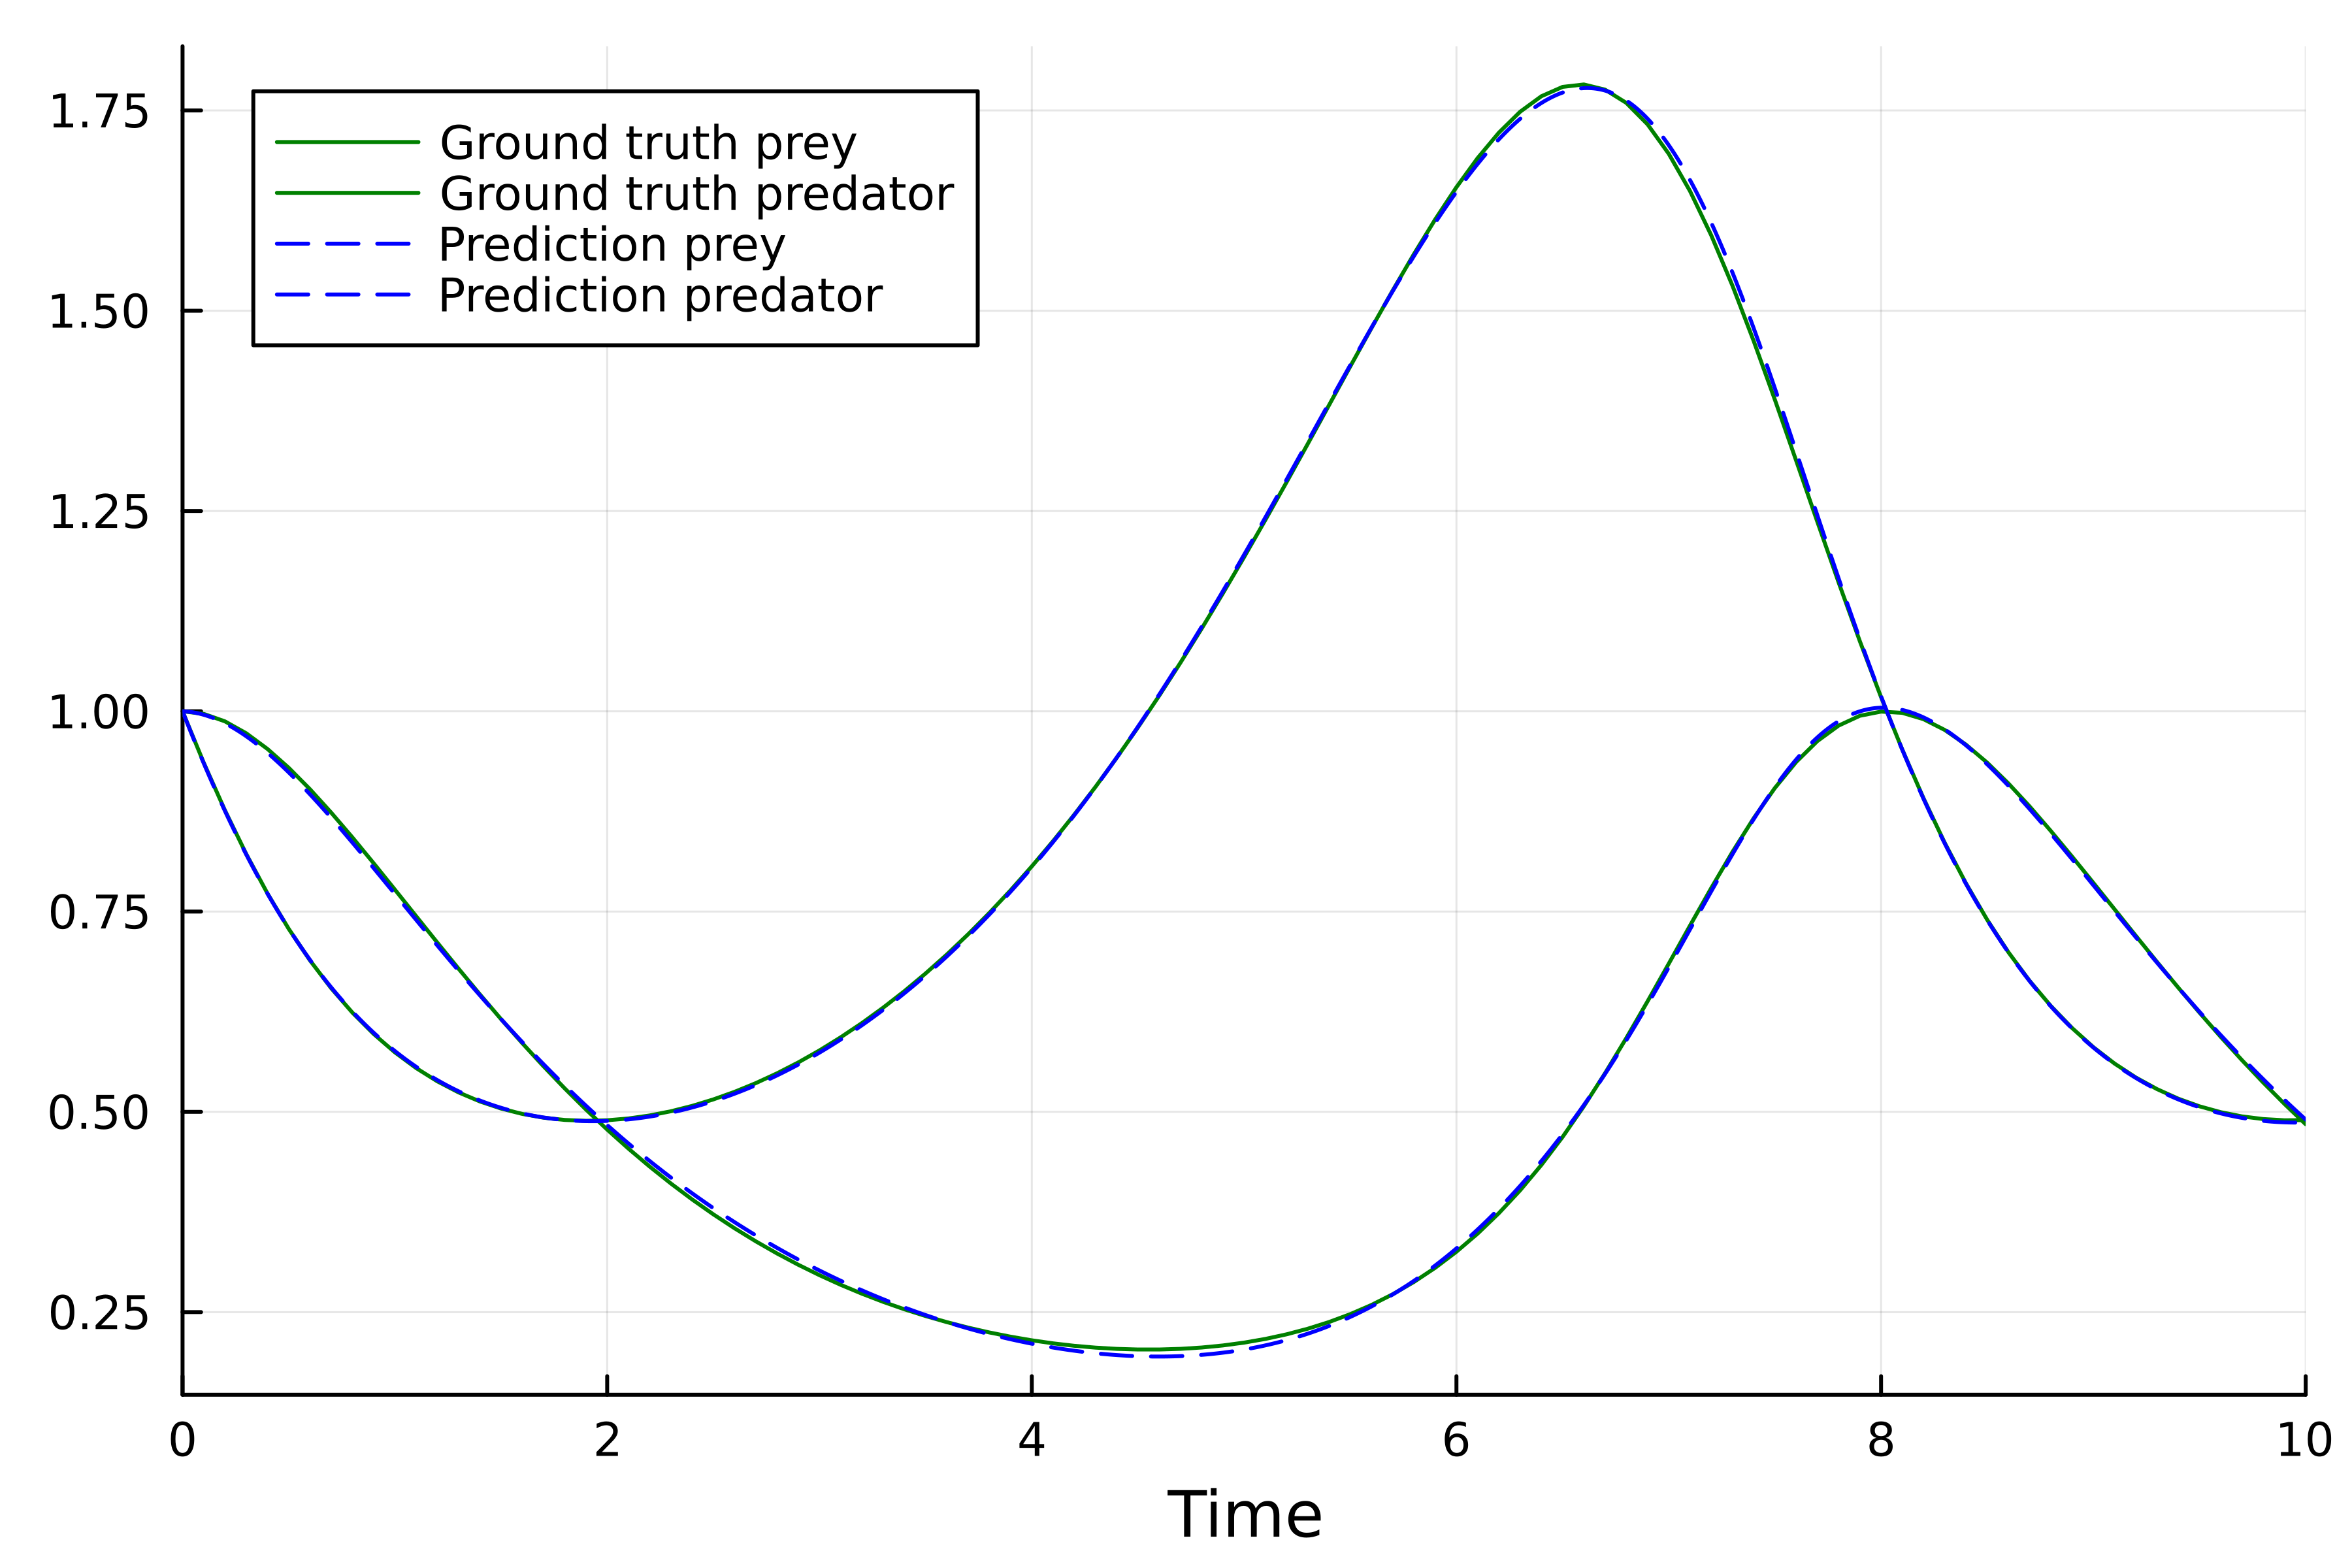
\includegraphics[width=0.5\linewidth]{../examples/lotka_volterra/comparison}
	\caption{Example \ref{ex:lotka_volterra}. Comparison between the true solution and our Neural ODE solution in the training interval $[0,10]$.}
	\label{fig:lotka_volterra_comparison}
\end{figure}

\begin{figure}[h!]
	\centering
	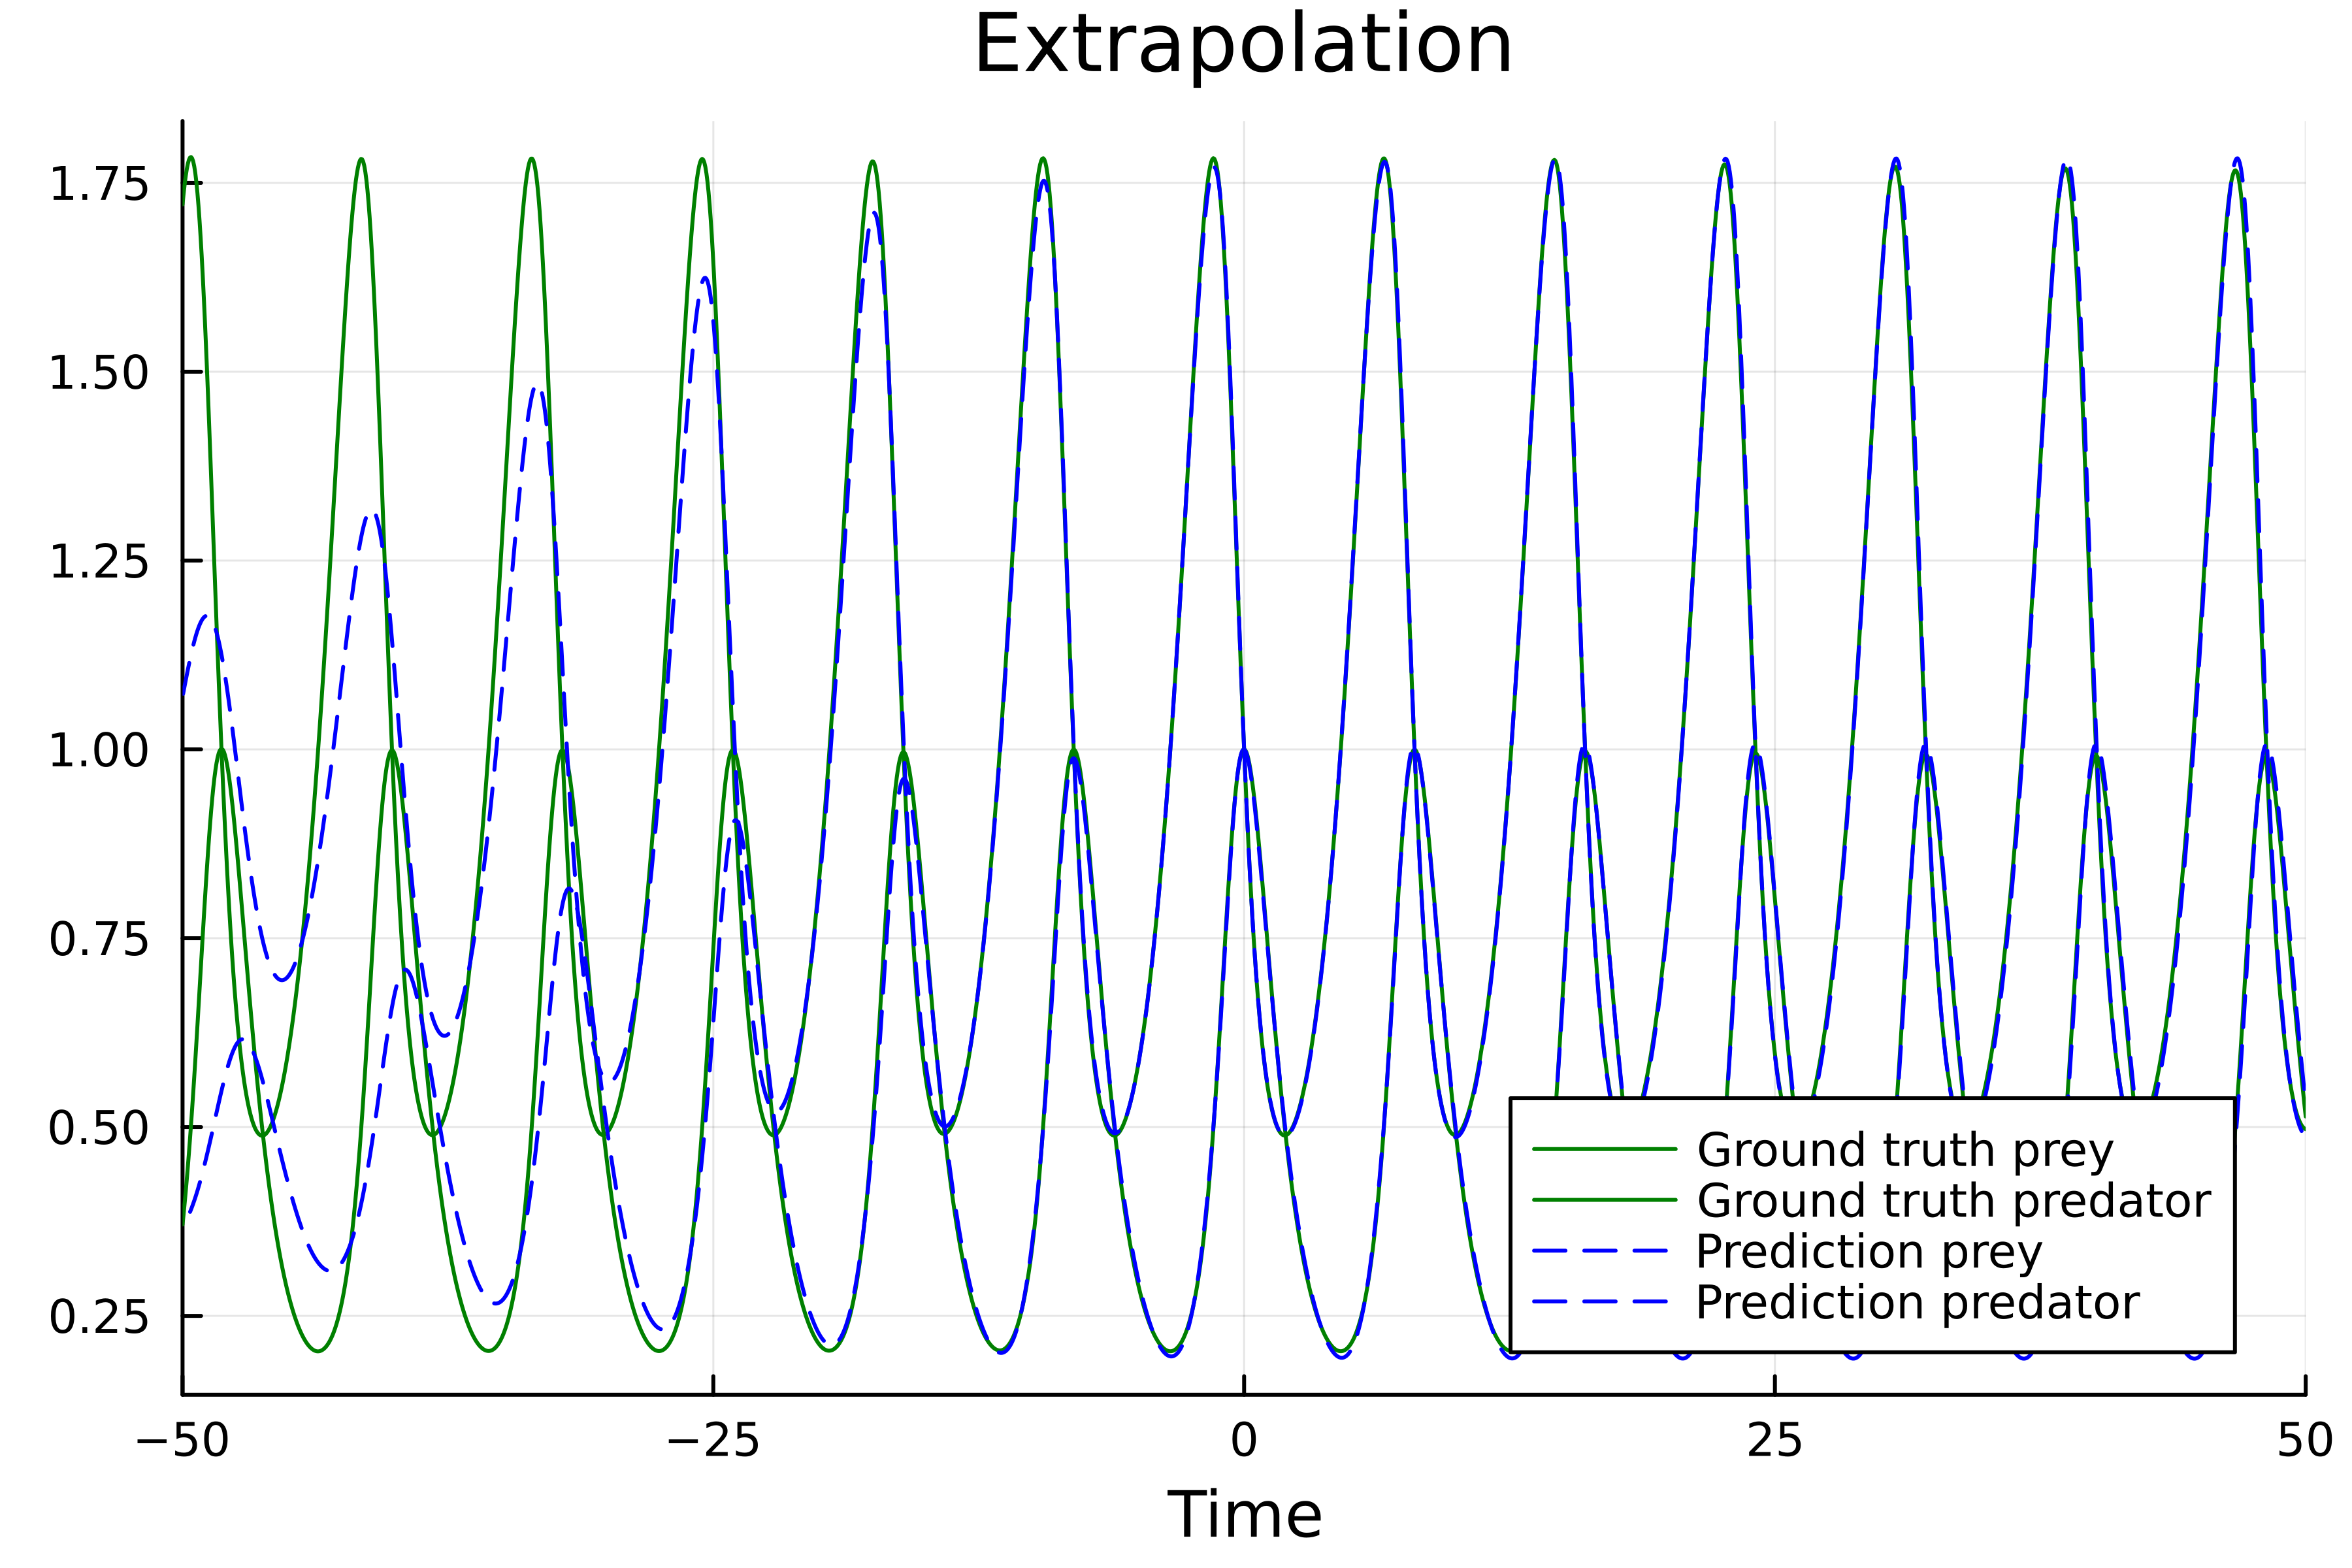
\includegraphics[width=0.5\linewidth]{../examples/lotka_volterra/extrapolation}
	\caption{Example \ref{ex:lotka_volterra}. Extrapolation of the ODE and Neural ODE solution outside the training interval.}
	\label{fig:lotka_volterra_extrapolation}
\end{figure}

\subsection{Example: Lotka-Volterra equations with noise}\label{ex:lotka_volterra_noisy}
In this example we test the performance of the Neural ODE when the observations contain noise. Here, we take the same Lotka-Volterra eqs. and parameters of Sec. \ref{ex:lotka_volterra}, but we add white gaussian noise $\eta\sim \mathcal{N}(\mu=0,\sigma=0.1)$ to each of the observation points, and we reduce the number of observations from 101 to 41.

A comparison between the true solution, the noisy observations and our Neural ODE solution in the training interval is shown in Fig. \ref{fig:lotka_volterra_noisy_comparison}, and a comparison outside the training interval is shown in Fig. \ref{fig:lotka_volterra_noisy_extrapolation}. We observe that the Neural ODE possess robustness to noise, since it is still able to follow closely the true solution and replicate its periodic behavior, even in the presence of noisy observations.

\begin{figure}[h!]
	\centering
	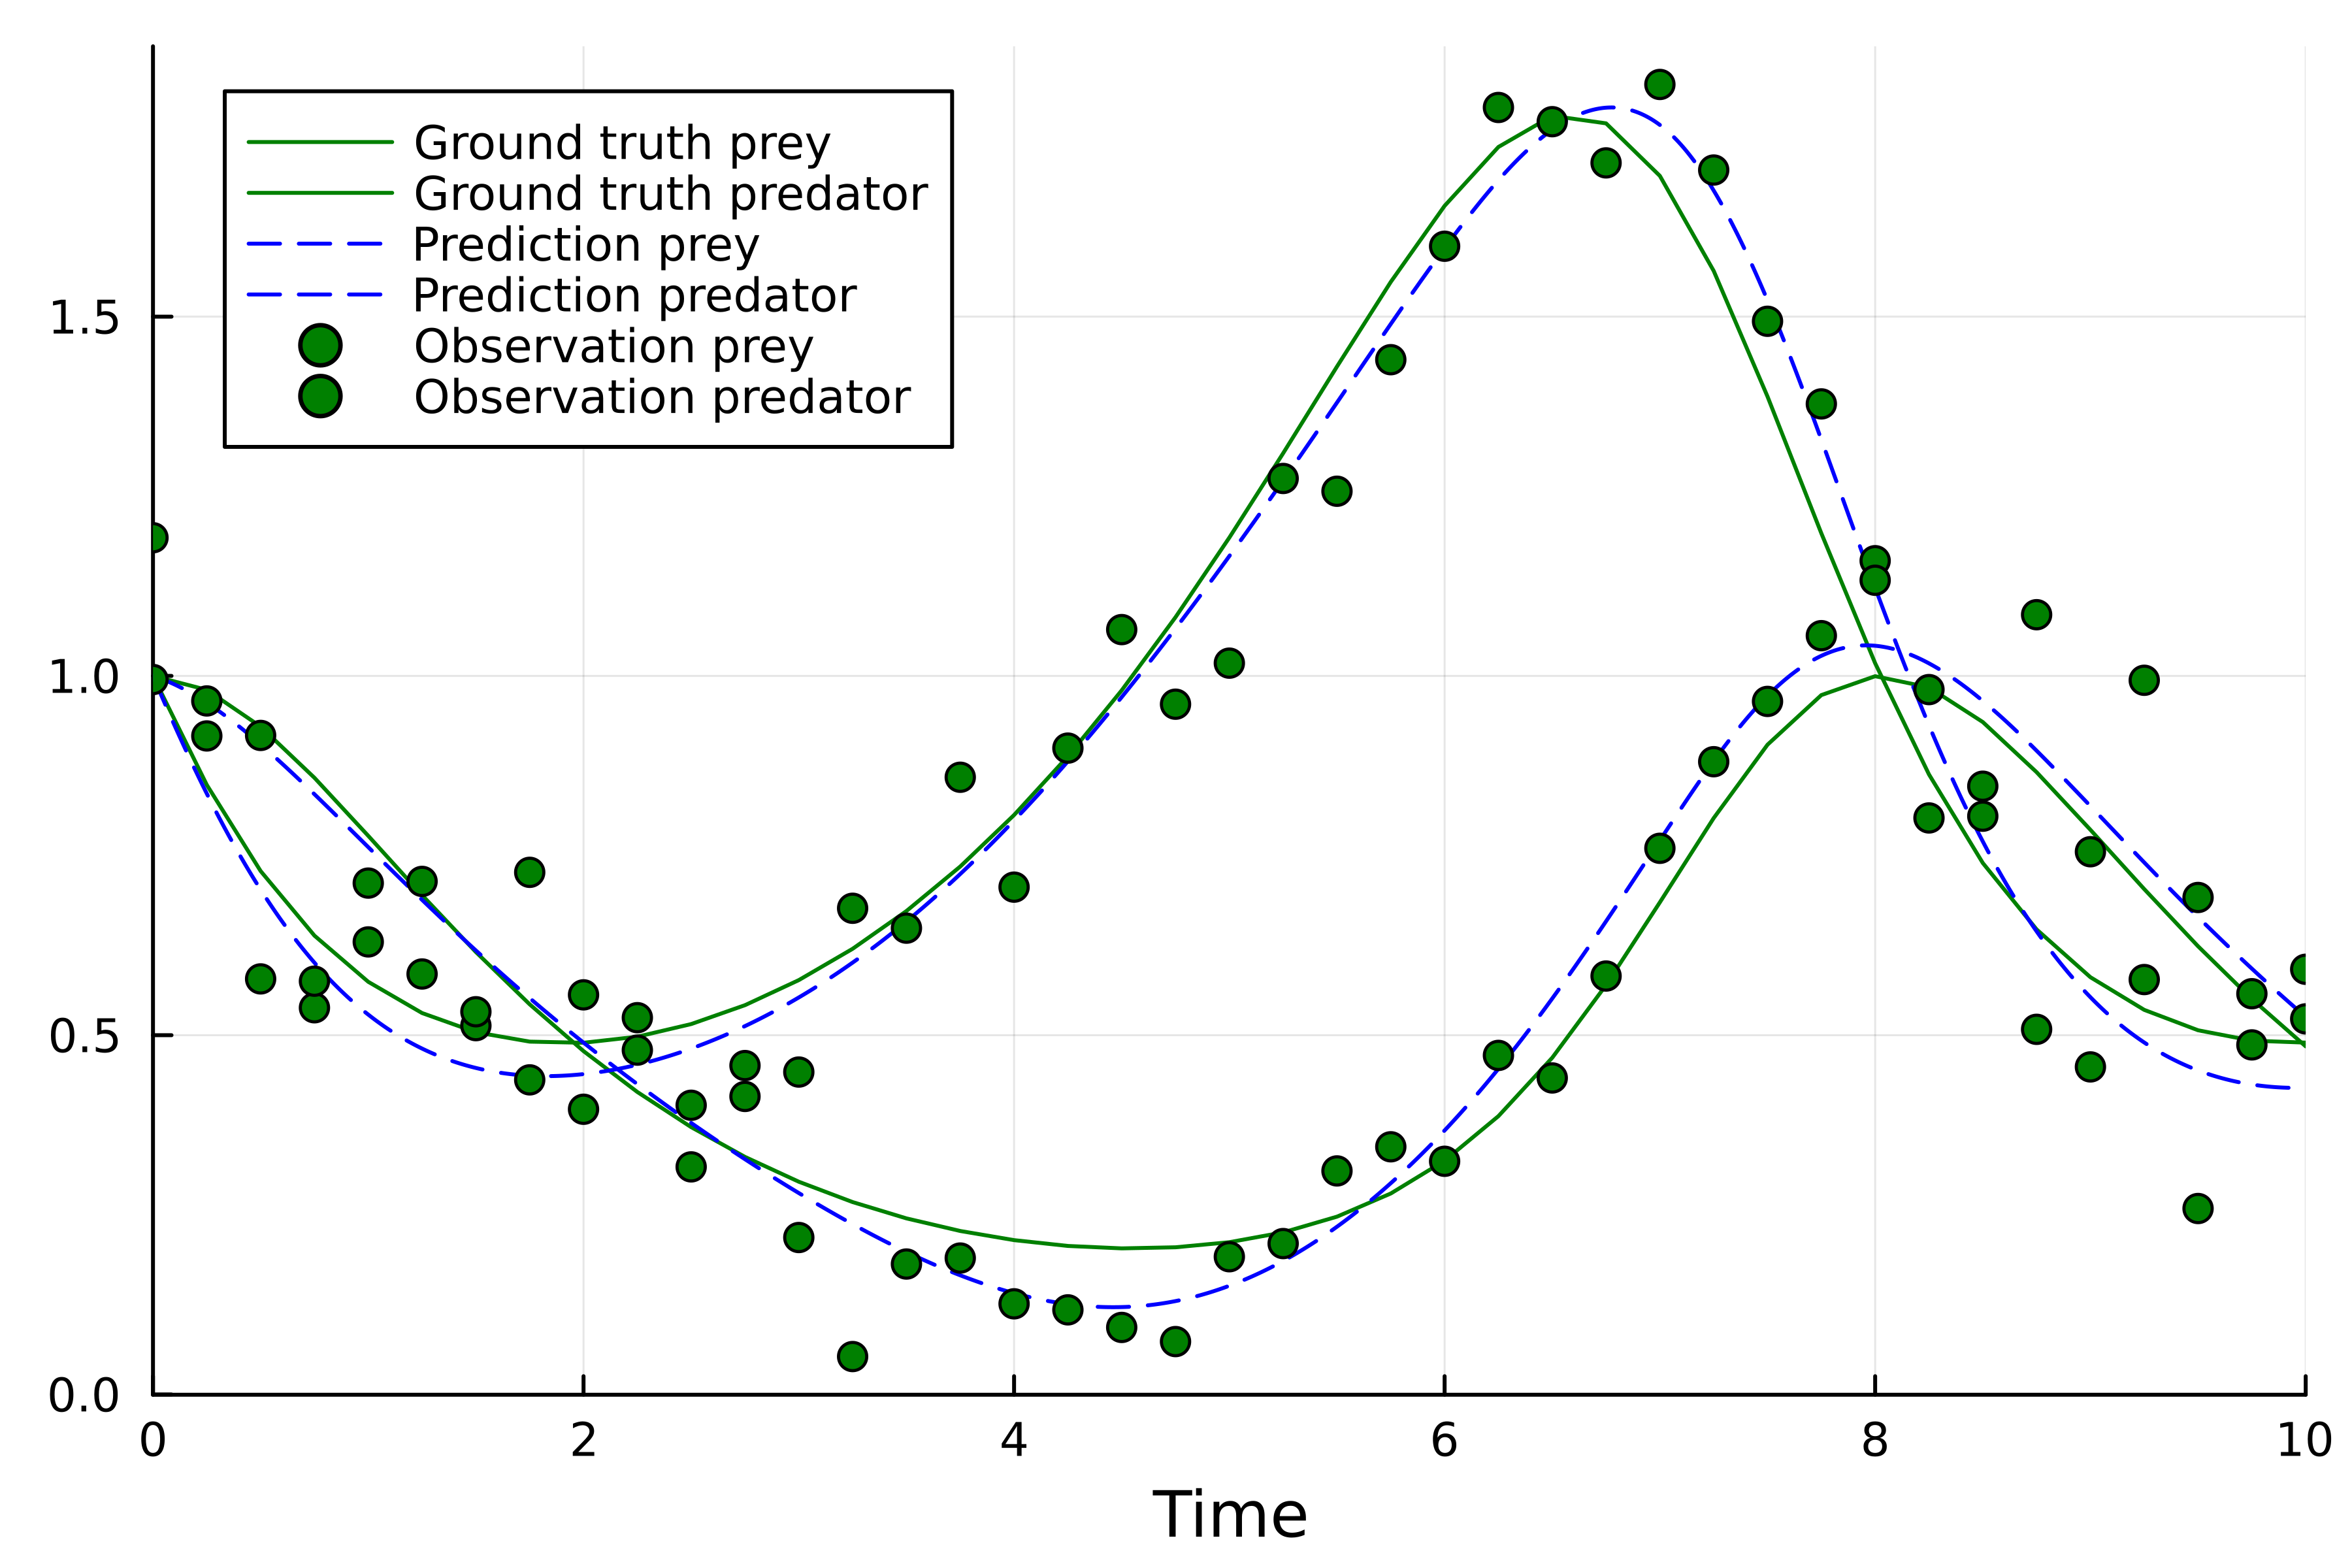
\includegraphics[width=0.5\linewidth]{../examples/lotka_volterra_noisy/comparison_01}
	\caption{Example \ref{ex:lotka_volterra_noisy}. Comparison between the true solution, the noisy observations and our Neural ODE solution in the training interval $[0,10]$.}
	\label{fig:lotka_volterra_noisy_comparison}
\end{figure}

\begin{figure}[h!]
	\centering
	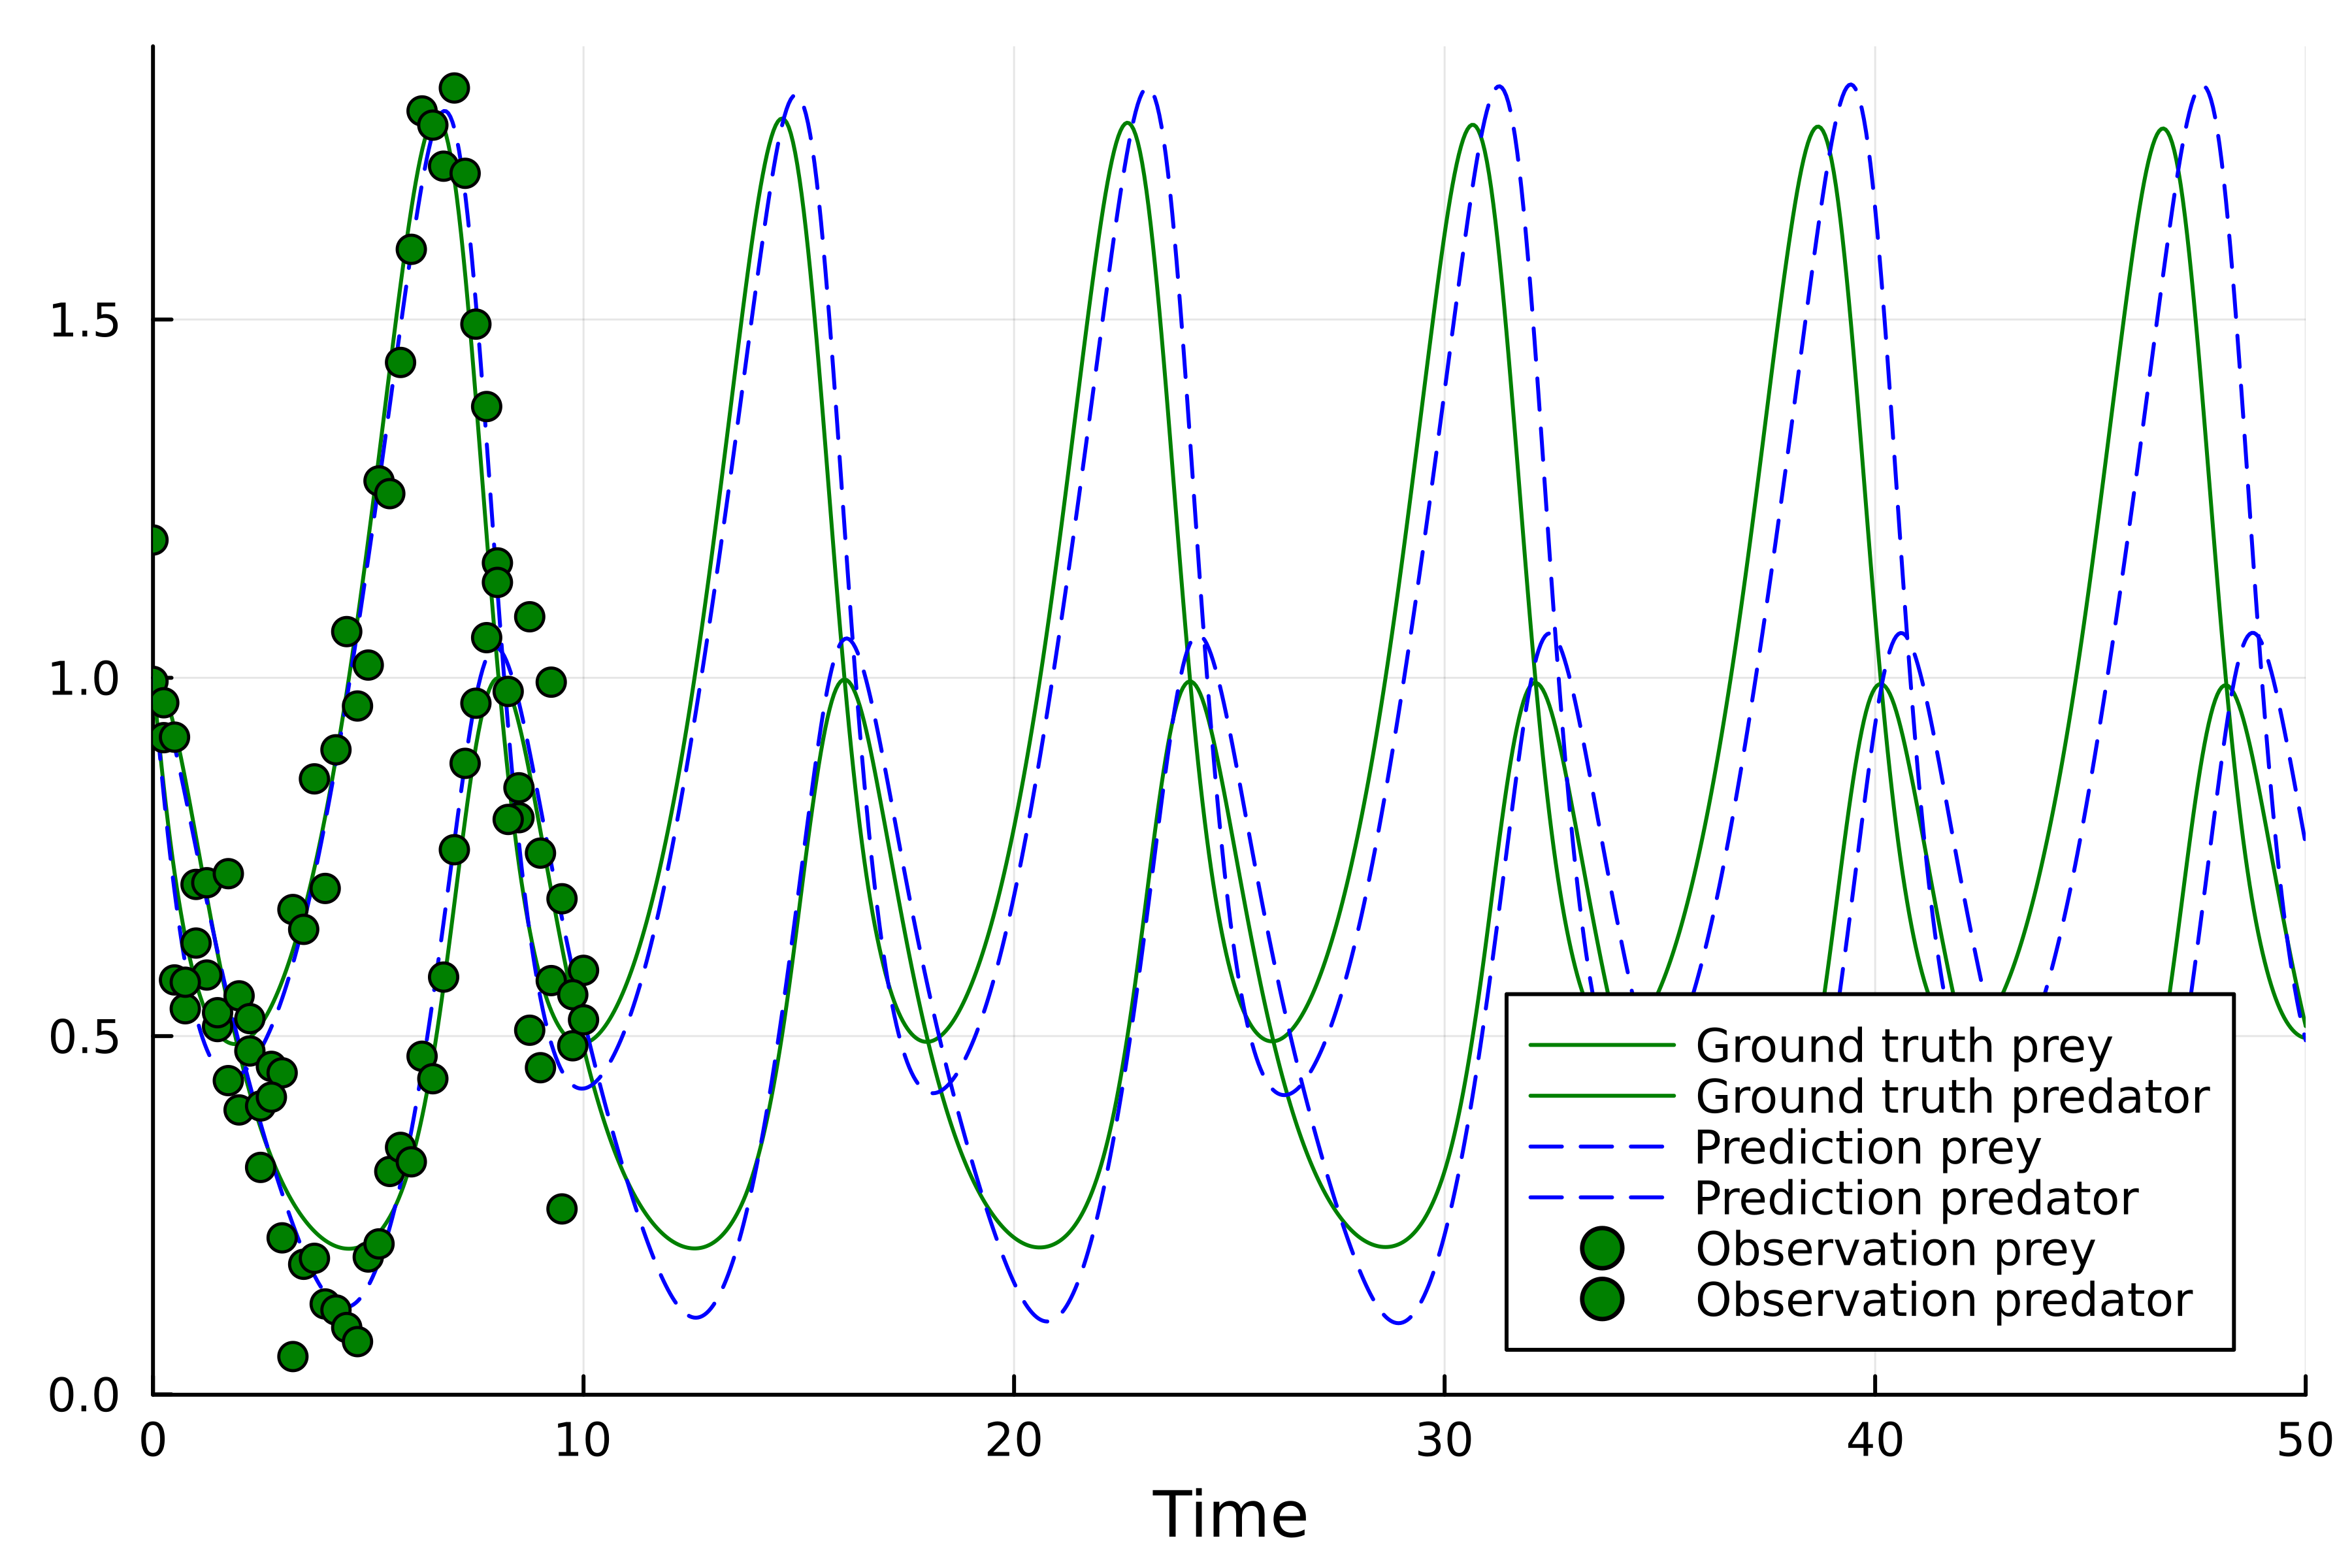
\includegraphics[width=0.5\linewidth]{../examples/lotka_volterra_noisy/extrapolation_01}
	\caption{Example \ref{ex:lotka_volterra_noisy}. Extrapolation of the ODE and Neural ODE solution outside the training interval. The noisy observations inside the training interval are also shown.}
	\label{fig:lotka_volterra_noisy_extrapolation}
\end{figure}

\subsection{Example: double pendulum}\label{ex:double_pendulum}
In this example we consider the dynamics of a double pendulum, as depicted in Fig. \ref{fig:double_pendulum}. Following the Hamiltonian formalism of classical mechanics, we have that the double pendulum has a Hamiltonian given by

\begin{align}
	H(\bol q,\bol p)=\frac{m_2 l_2^2 p_{\theta_1}^2+\left(m_1+m_2\right) l_1^2 p_{\theta_2}^2-2 m_2 l_1 l_2 p_{\theta_1} p_{\theta_2} \cos \left(\theta_1-\theta_2\right)}{2 m_2 l_1^2 l_2^2\left[m_1+m_2 \sin ^2\left(\theta_1-\theta_2\right)\right]} \notag\\
	-\left(m_1+m_2\right) g l_1 \cos \theta_1-m_2 g l_2 \cos \theta_2, \label{eq:hamil}
\end{align}
where $\bol q = (\theta_1,\theta_2)$ are the pendulums angles, $\bol p =(p_{\theta_1}, p_{\theta_2})$ the canonical momenta of the system, $(m_1,m_2)$ the pendulum masses, $(l_1,l_2)$ the pendulum lengths and $g$ the gravitational acceleration. The canonical momenta $(p_{\theta_1}, p_{\theta_2})$ have analytical expressions given in terms of $(\theta_1,\theta_2,\dot{\theta}_1,\dot{\theta}_2)$, but those expressions are not relevant for our purposes. The dynamics of the double pendulum follow Hamilton's equations, given by
\begin{subequations}
\begin{align}
	\frac{d\bol{q}}{dt} &= \frac{\partial H(\bol q,\bol p)}{\partial \bol{p}},\\
	\frac{d\bol{p}}{dt} &= -\frac{\partial H(\bol q,\bol p)}{\partial \bol{q}}.
\end{align} \label{eq:hamilton_eq}
\end{subequations}


The double pendulum equations are nonlinear, exhibit chaotic behavior, and the solutions are in general aperiodic.

We compared the true ODE solution against a Neural ODE trained in the interval $[0,0.25]$ with initial conditions $\bol q = (0.05,-0.05)$, $\bol p =(0,0)$ and 26 uniformly spaced observations. We took $(m_1,m_2,l_1,l_2,g) = (1,1,1,1,9.8)$. Our results are shown in Figs. \ref{fig:double_pendulum_comparison} and \ref{fig:double_pendulum_extrapolation}, for comparisons inside and outside the training interval, respectively. As in the previous examples, the Neural ODE is able to follow the true solution inside the training interval, and even replicate the aperiodic and complex behavior outside of it.

In a Hamiltonian system, such as the double pendulum, if Hamiltonian \eqref{eq:hamil} is independent of time, then the Hamiltonian itself must be a conserved quantity. A comparison of the Hamiltonians of the true ODE and the Neural ODE is shown in Fig. \ref{fig:double_pendulum_hamiltonian}. Although in theory the Hamiltonian of the true ODE solution should be conserved, we see it is not the case, in fact, it is slowing increasing. This is due to the ODE solver, which is not designed to conserve the Hamiltonian over time. A class of ODE solvers denominated symplectic solvers are able to maintain conserved quantities over time \cite{leimkuhler2004simulating}, but they were not used in this work. 

In the Neural ODE case we observe the Hamiltonian decreases over time, it is not conserved. This is mainly due to the fact that Neural ODE does not follow a Hamiltonian structure, such as \ref{eq:hamilton_eq}, hence the Hamiltonian is not necessary conserved. This poses a challenge as it enables the Neural ODE to evolve towards prohibited states. The system's allowed states are limited to those that possess the same Hamiltonian value as the initial condition. We will explain in Sec. \ref{sec:hnn} how this difficulty can be overcome with the use of Hamiltonian Neural Networks.

\begin{figure}[h!]
	\centering
	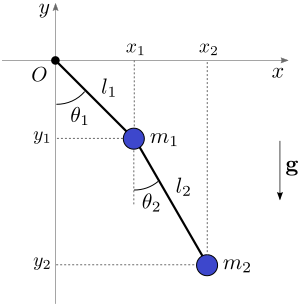
\includegraphics[width=0.4\linewidth]{double-pendulum}
	\caption{Example \ref{ex:double_pendulum}. Schematic of a double pendulum.}
	\label{fig:double_pendulum}
\end{figure}

\begin{figure}[h!]
	\centering
	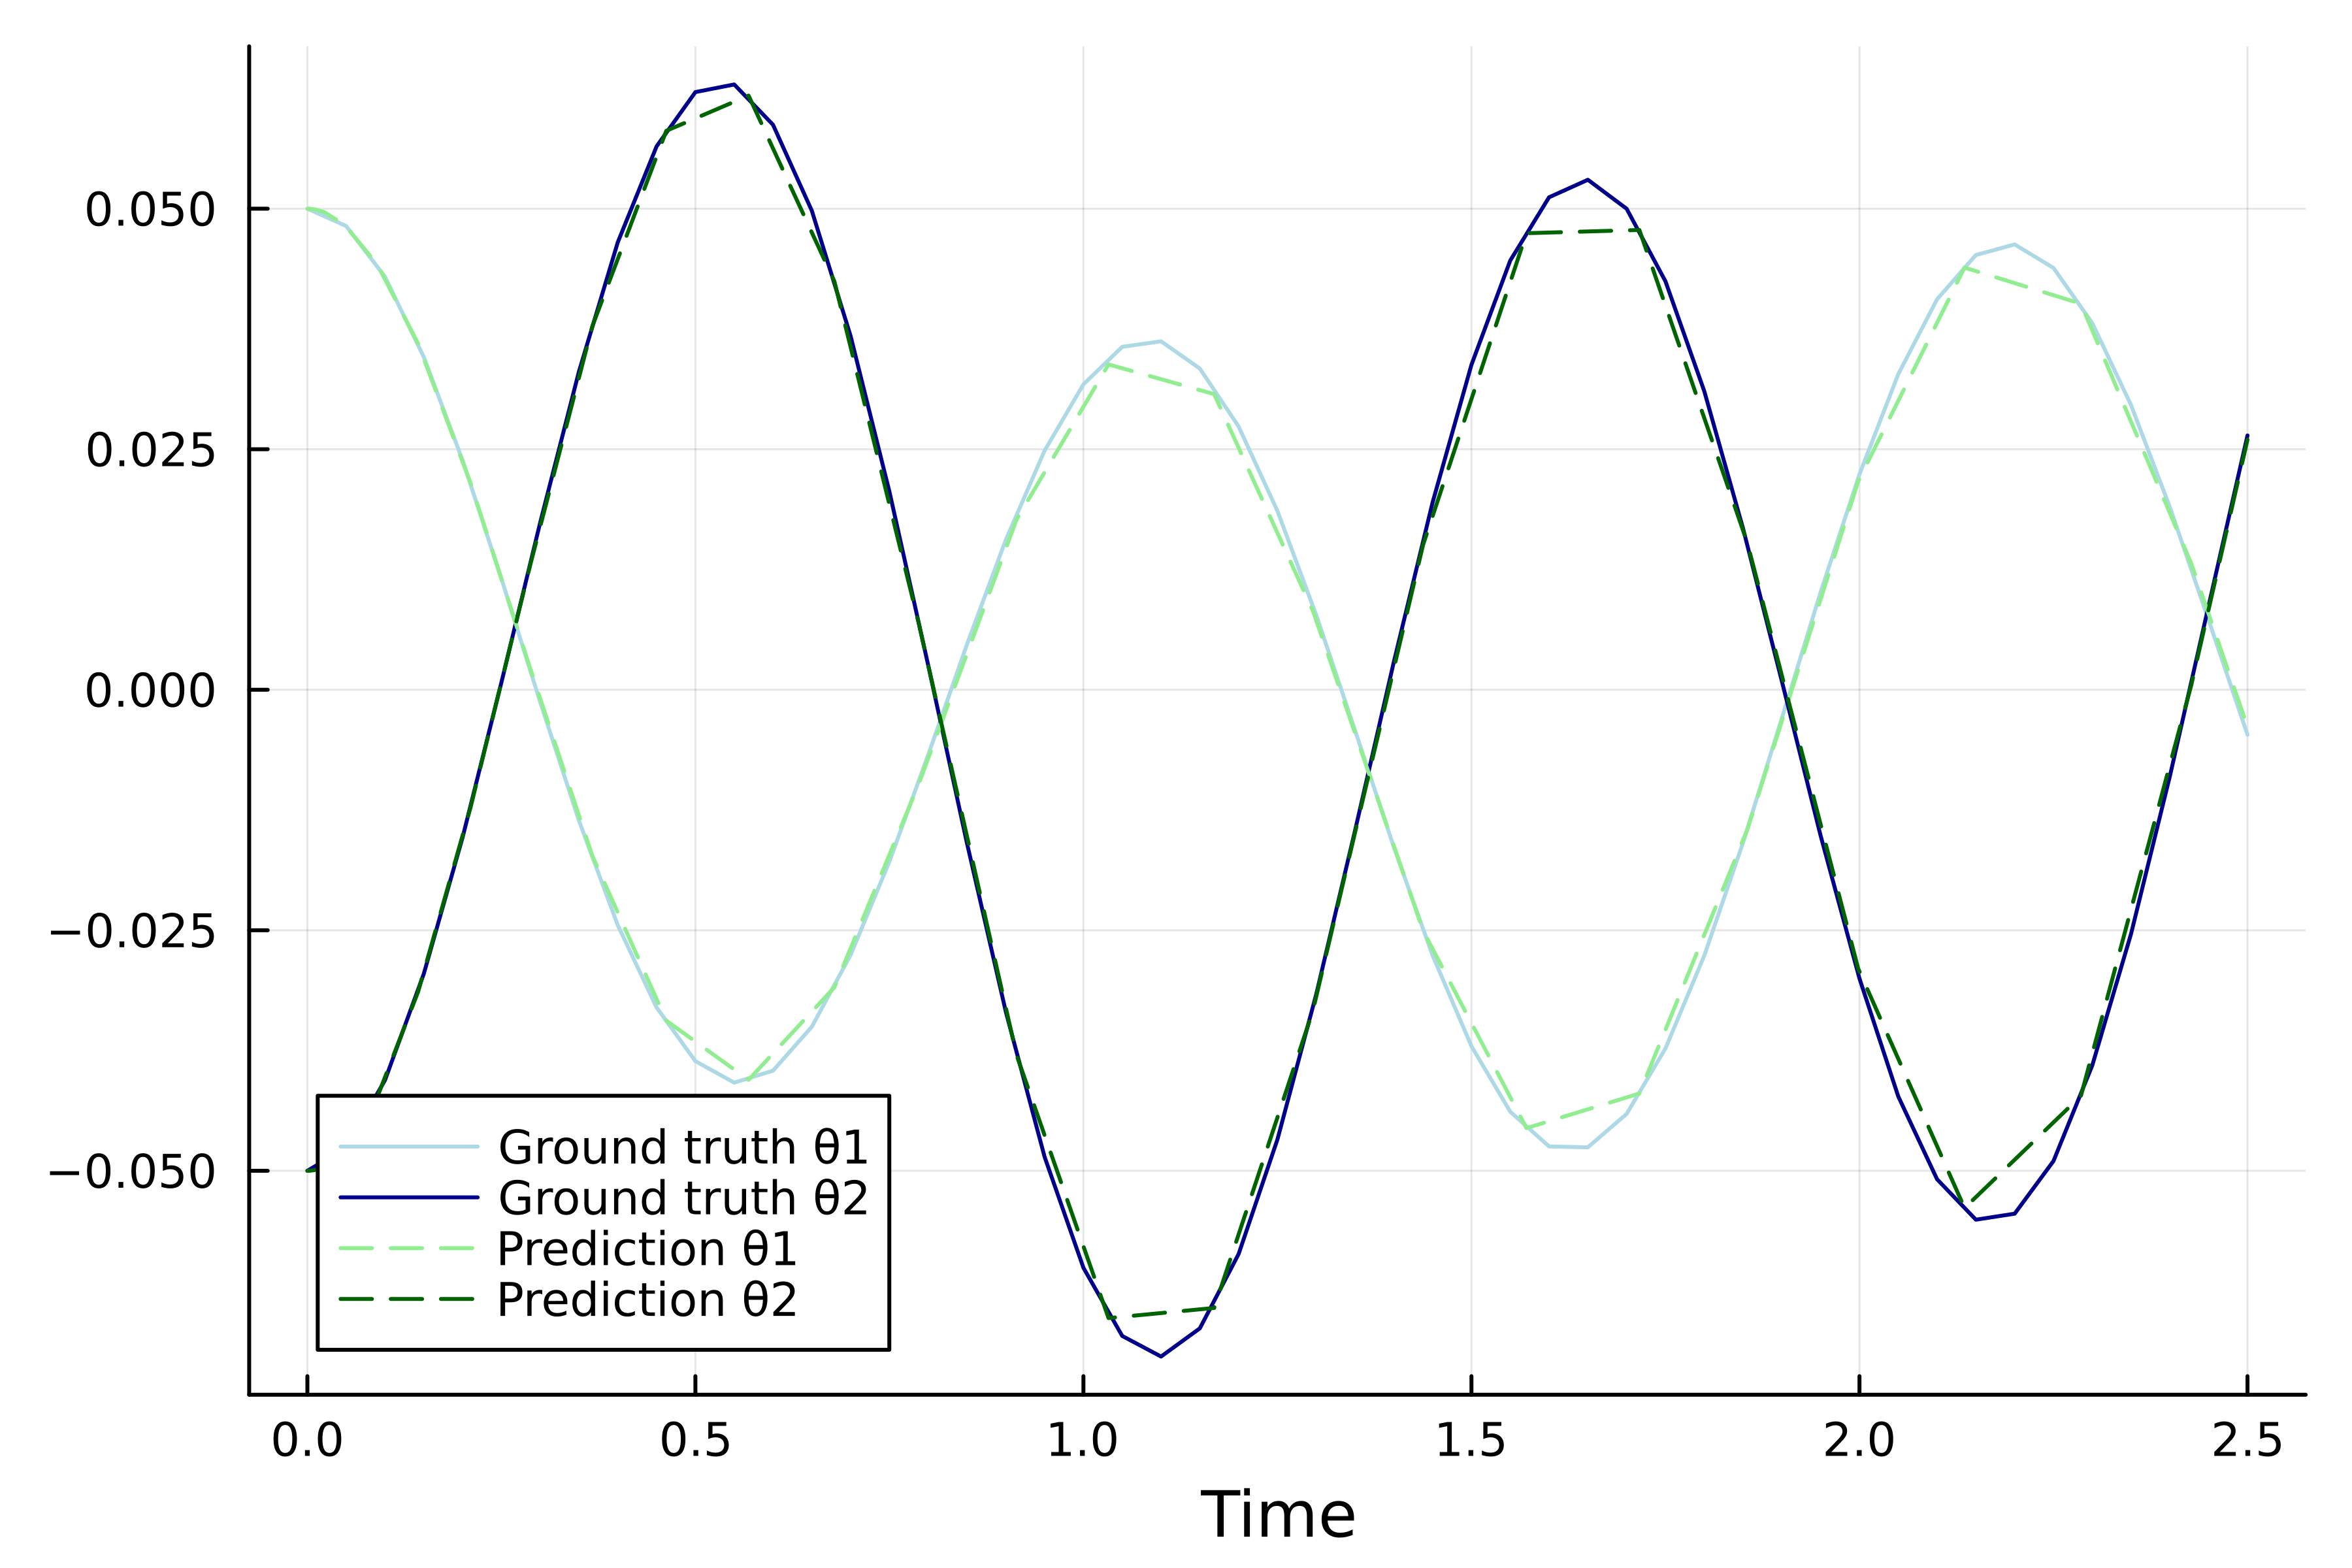
\includegraphics[width=0.5\linewidth]{../examples/double_pendulum/comparison}
	\caption{Example \ref{ex:double_pendulum}. Comparison between the true solution and our Neural ODE solutions in the training interval $[0,10]$.}
	\label{fig:double_pendulum_comparison}
\end{figure}

\begin{figure}[h!]
	\centering
	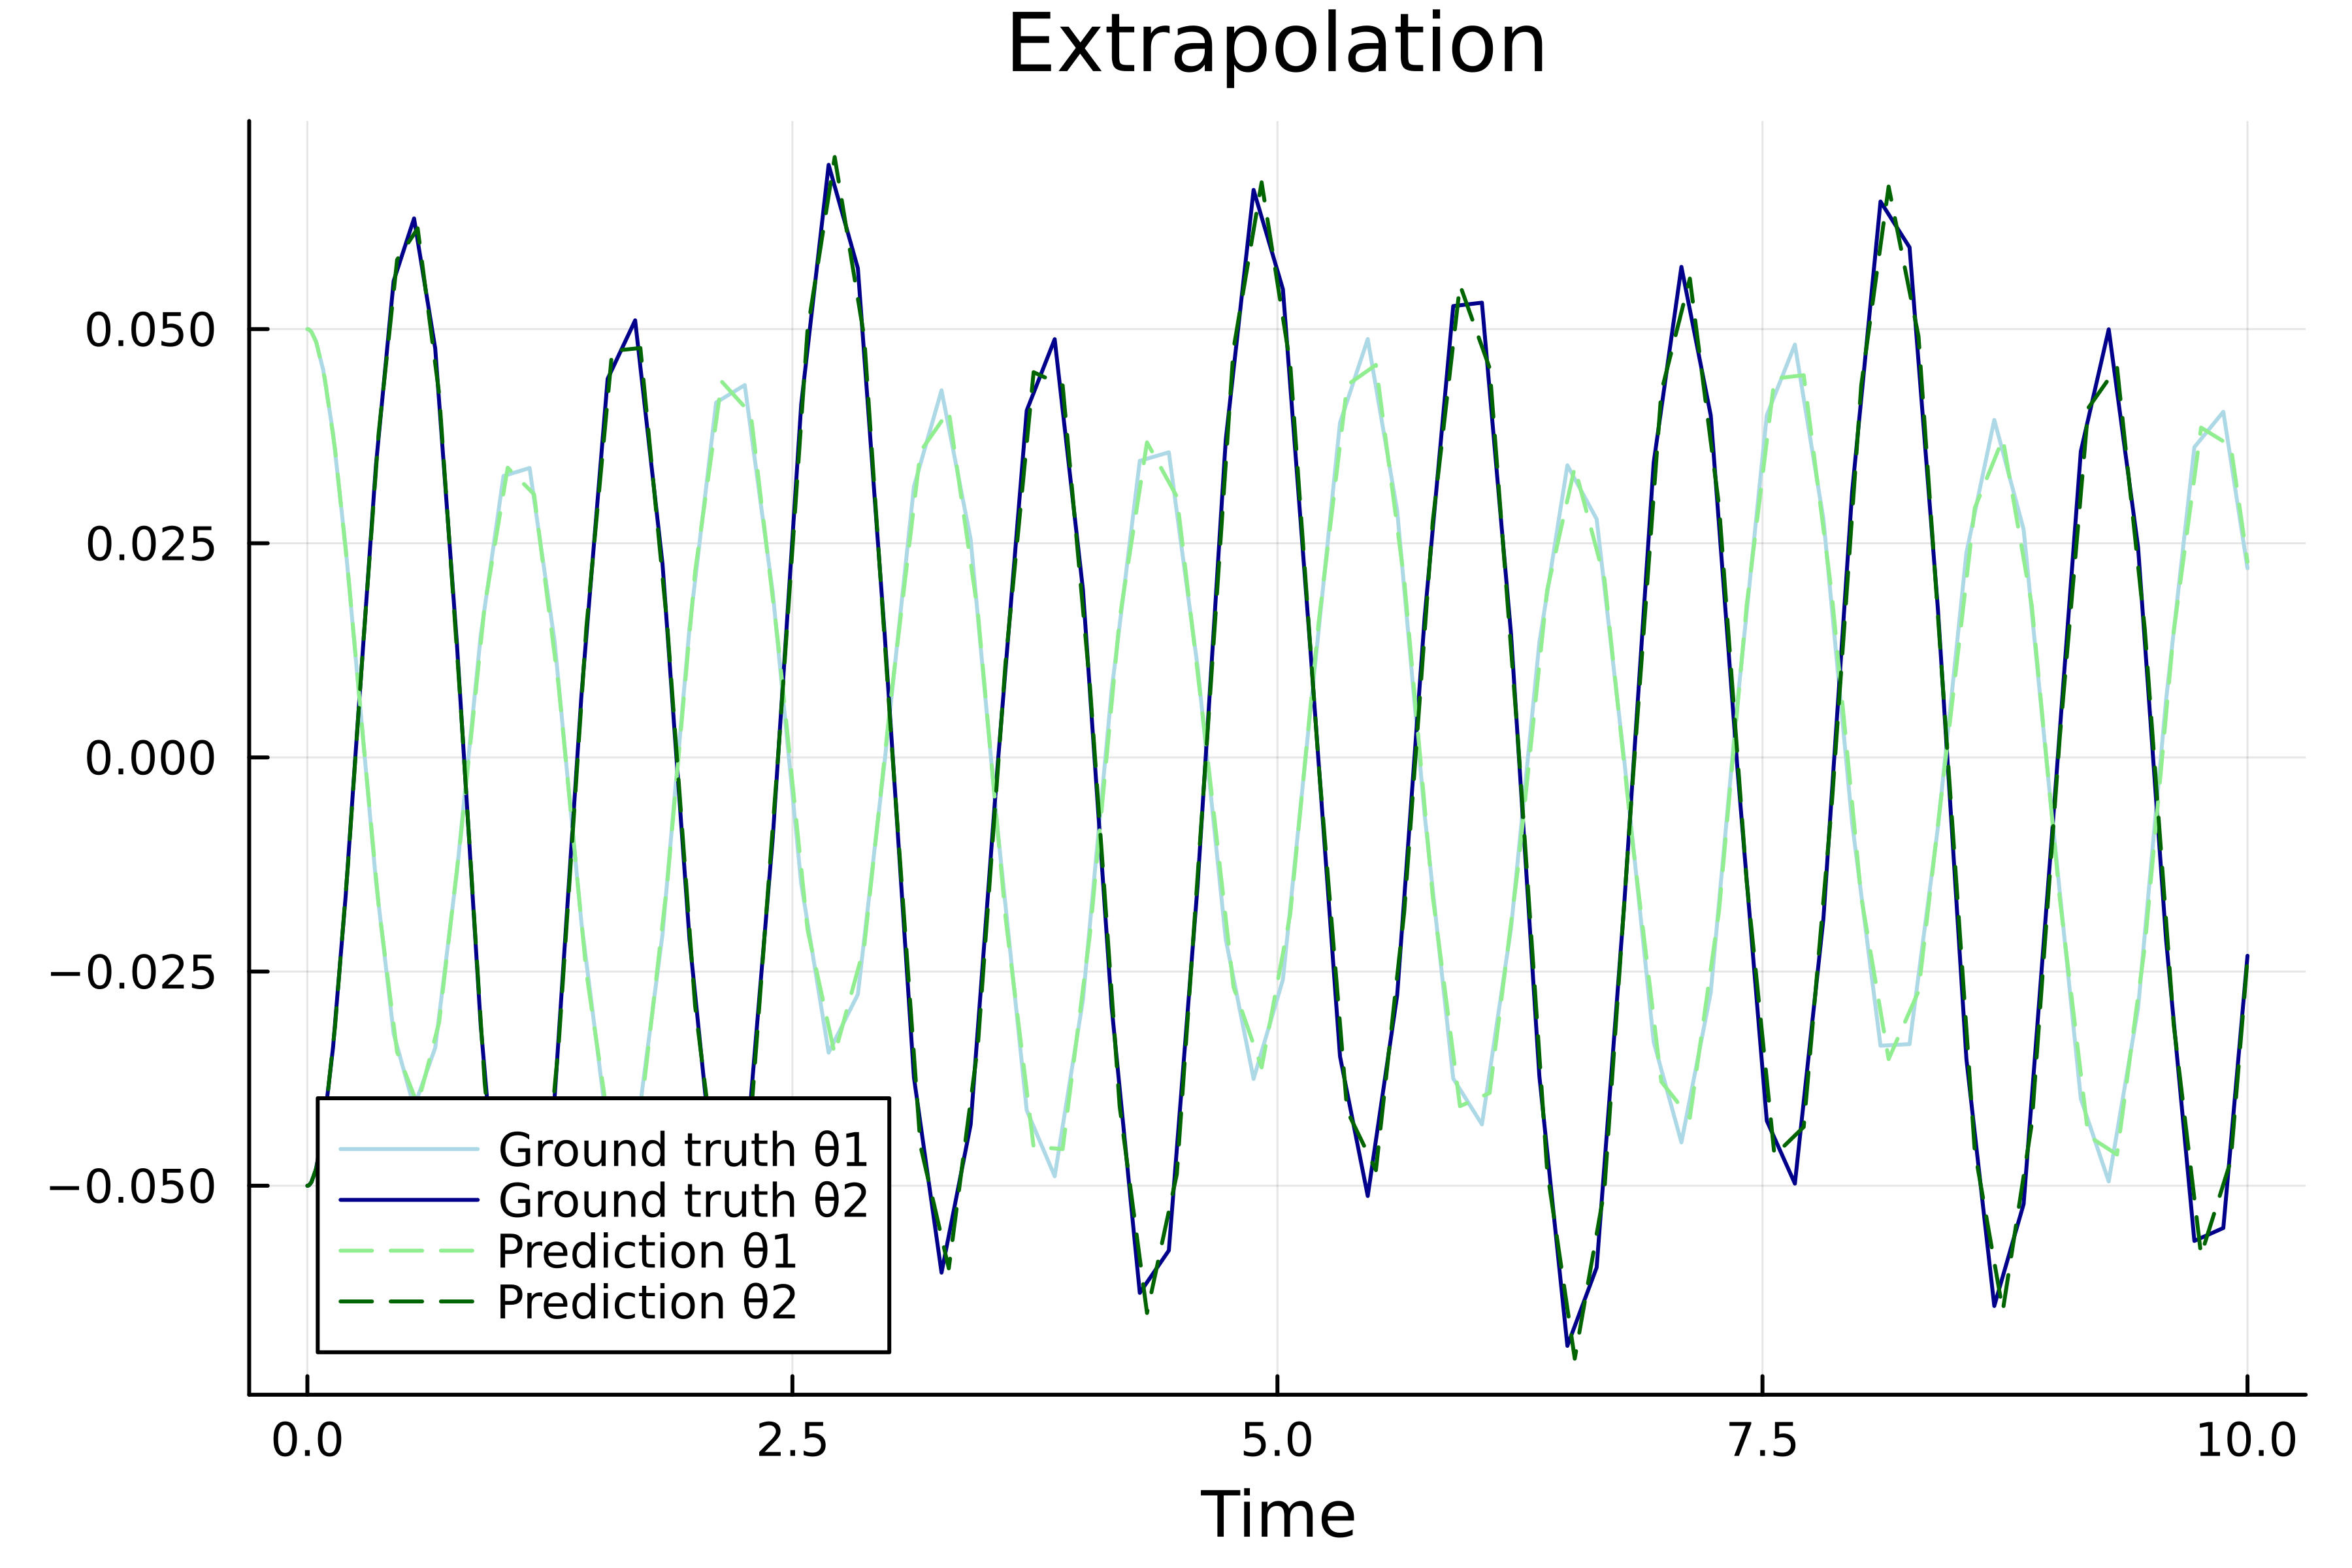
\includegraphics[width=0.5\linewidth]{../examples/double_pendulum/extrapolation}
	\caption{Example \ref{ex:double_pendulum}. Extrapolation of the ODE and Neural ODE solutions outside the training interval.}
	\label{fig:double_pendulum_extrapolation}
\end{figure}

\begin{figure}[h!]
	\centering
	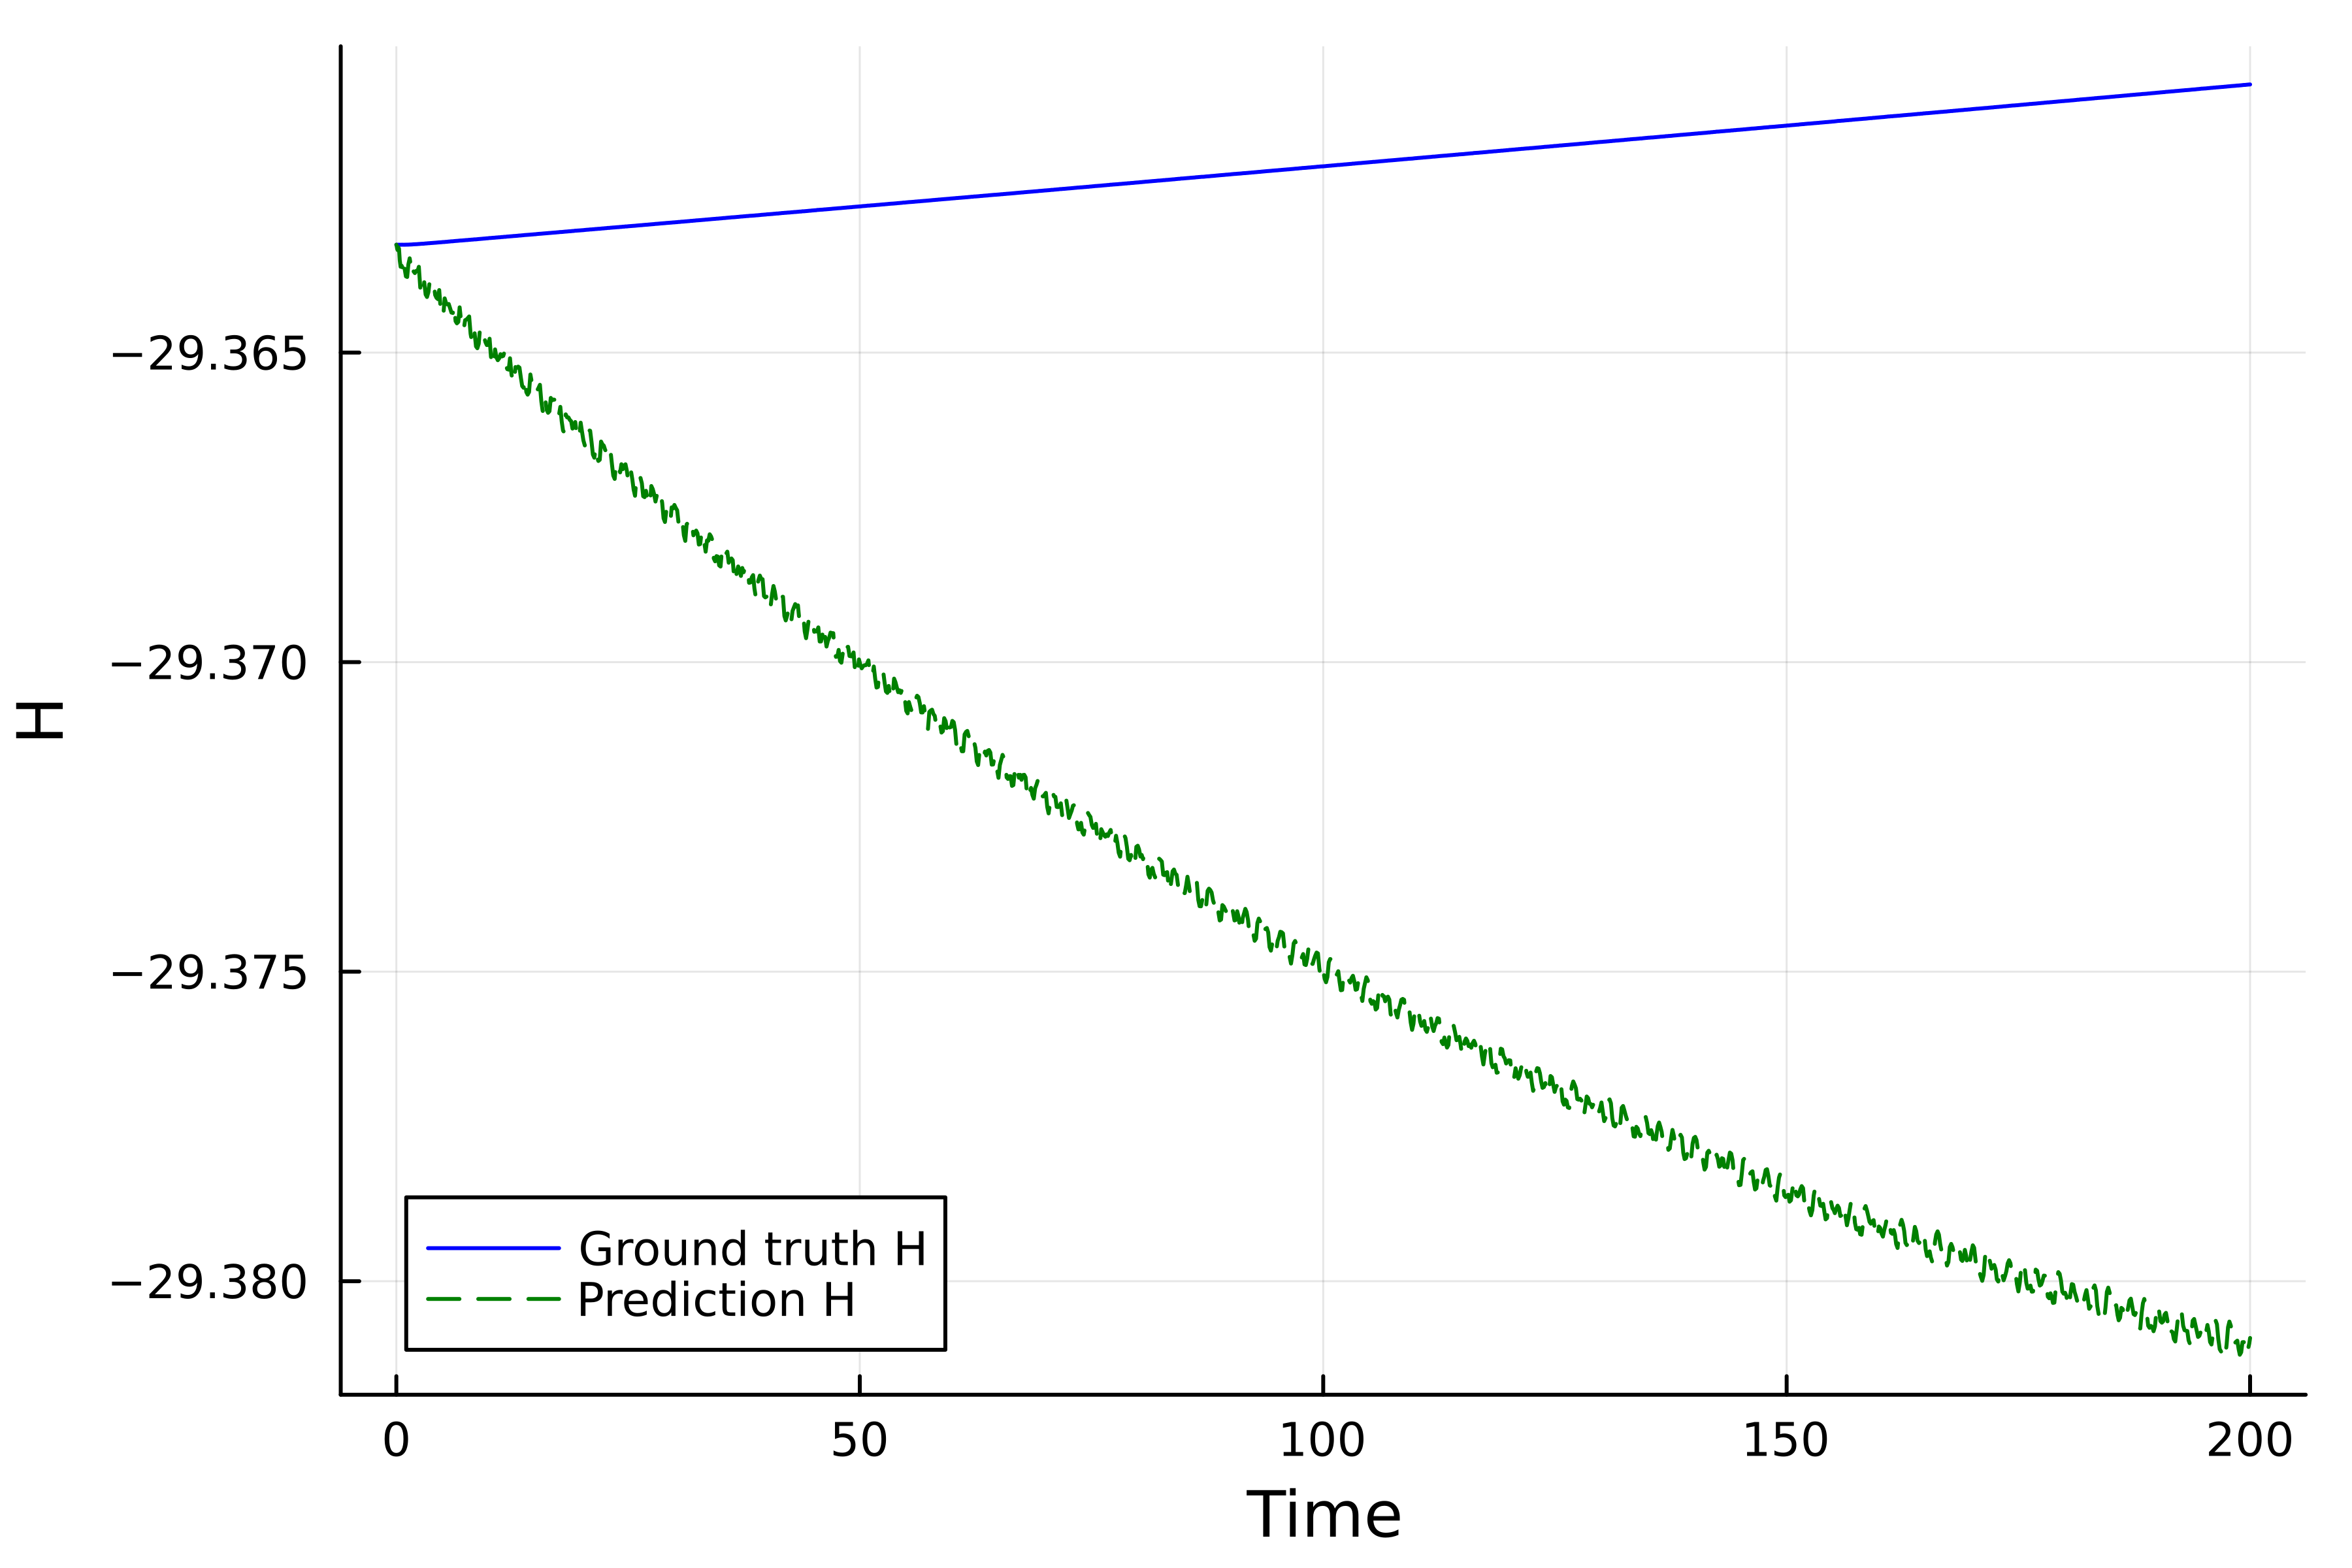
\includegraphics[width=0.5\linewidth]{../examples/double_pendulum/hamiltonian}
	\caption{Example \ref{ex:double_pendulum}. Hamiltonian of ODE and Neural ODE solutions outside the training interval.}
	\label{fig:double_pendulum_hamiltonian}
\end{figure}

\section{Hamiltonian Neural Networks}\label{sec:hnn}
Hamiltonian Neural Networks (HNNs) are a subclass of Neural ODEs specifically design to deal with Hamiltonian system, proposed by Greydanus et at. in 2019\cite{greydanus2019hamiltonian}. Unlike the Neural ODEs approach, which would replace the right-hand-side of Hamilton's eqs. \eqref{eq:hamilton_eq} with a neural network, in HNNs the Hamiltonian itself is modeled with a neural network, this is
\begin{align}
	H(\bol q, \bol p) = \text{NN}(\bol q, \bol p,\bol \theta),
\end{align}
and thus Hamilton's eqs. now read
\begin{subequations}
	\begin{align}
		\frac{d\bol{q}}{dt} &= \frac{\partial}{\partial \bol{p}}\text{NN}(\bol q, \bol p,\bol \theta),\\
		\frac{d\bol{p}}{dt} &= -\frac{\partial}{\partial \bol{q}}\text{NN}(\bol q, \bol p,\bol \theta).
	\end{align}\label{eq:hnn_eq}
\end{subequations}

The fact that HNNs preserve the underlying Hamiltonian structure of the system lead to unique advantages, such as the (theoretical) conservation energy and long-term stability, useful in accurate long-term predictions.

Some difficulties of HNNs are, first, that in order to perform backpropagation we require to take second order derivatives of our neural network. To see this, note that we need first order derivatives in the forward pass (eq. \ref{eq:hnn_eq}), and then take derivatives one more time in the backward pass (eq. \ref{eq:adjointode}). This is expensive, and some automatic differentiation libraries, such as Zygote.jl, have limited capabilities with respect to second or higher order derivatives. Second, in some system it is not obvious how to compute or measure the canonical momenta $\bol p$, hence in those cases we cannot formulate the dynamics of the system of interest with the Hamiltonian formalism. An alternative to HNNs, namely Lagrangian Neural Networks \cite{cranmer2020lagrangian}, uses the Lagrangian formalism instead of the Hamiltonian formalism, and thus avoids the computation of canonical momenta, it only requires generalized coordinates $\bol q$ and generalized velocities $\dot{\bol{q}}$. Nevertheless, it presents other difficulties on its own: it requires third order derivatives and to solve linear systems in both the forward and backward passes.

\subsection{Example: hamiltonian double pendulum}\label{ex:hnn_double_pendulum}
Here we repeat Example \ref{ex:double_pendulum}, but using a HNN instead. This time we resort to the DiffEqFlux.jl package for a HNN implementation, instead of an in-house implementation of our own, just for showcasing purposes, and additionally because the Zygote.jl library presents difficulties to obtain second order derivatives of neural networks with respect to their weights, which are required for backpropagation. Furthermore, for simplicity we utilize the collocation method, detailed in \cite{roesch2021collocation}, to train the HNN.

The HNN is able to keep up with the true solution, both inside the training interval and forward in time, just like the Neural ODE counterpart. However, this time our model posses a Hamiltonian structure, hence the Hamiltonian should be conserved, at least theoretically. A comparison between the Hamiltonians of the ODE solution and the HNN is shown in Fig. \ref{fig:hnn_double_pendulum_hamiltonian}. We observe that both Hamiltonians grow slowly at the same rate. As pointed out in Example \ref{ex:double_pendulum}, this growing is due to numerical errors in the ODE solver, and not due to the lack of Hamiltonian structure. It can be said with certain then that our HNN is able to correctly reproduce the Hamiltonian structure of the system and to conserve the Hamiltonian. We are secure that, if we employed a symplectic solver, we would observe a constant Hamiltonian, in both the ODE and HNN solutions.

\begin{figure}[h!]
	\centering
	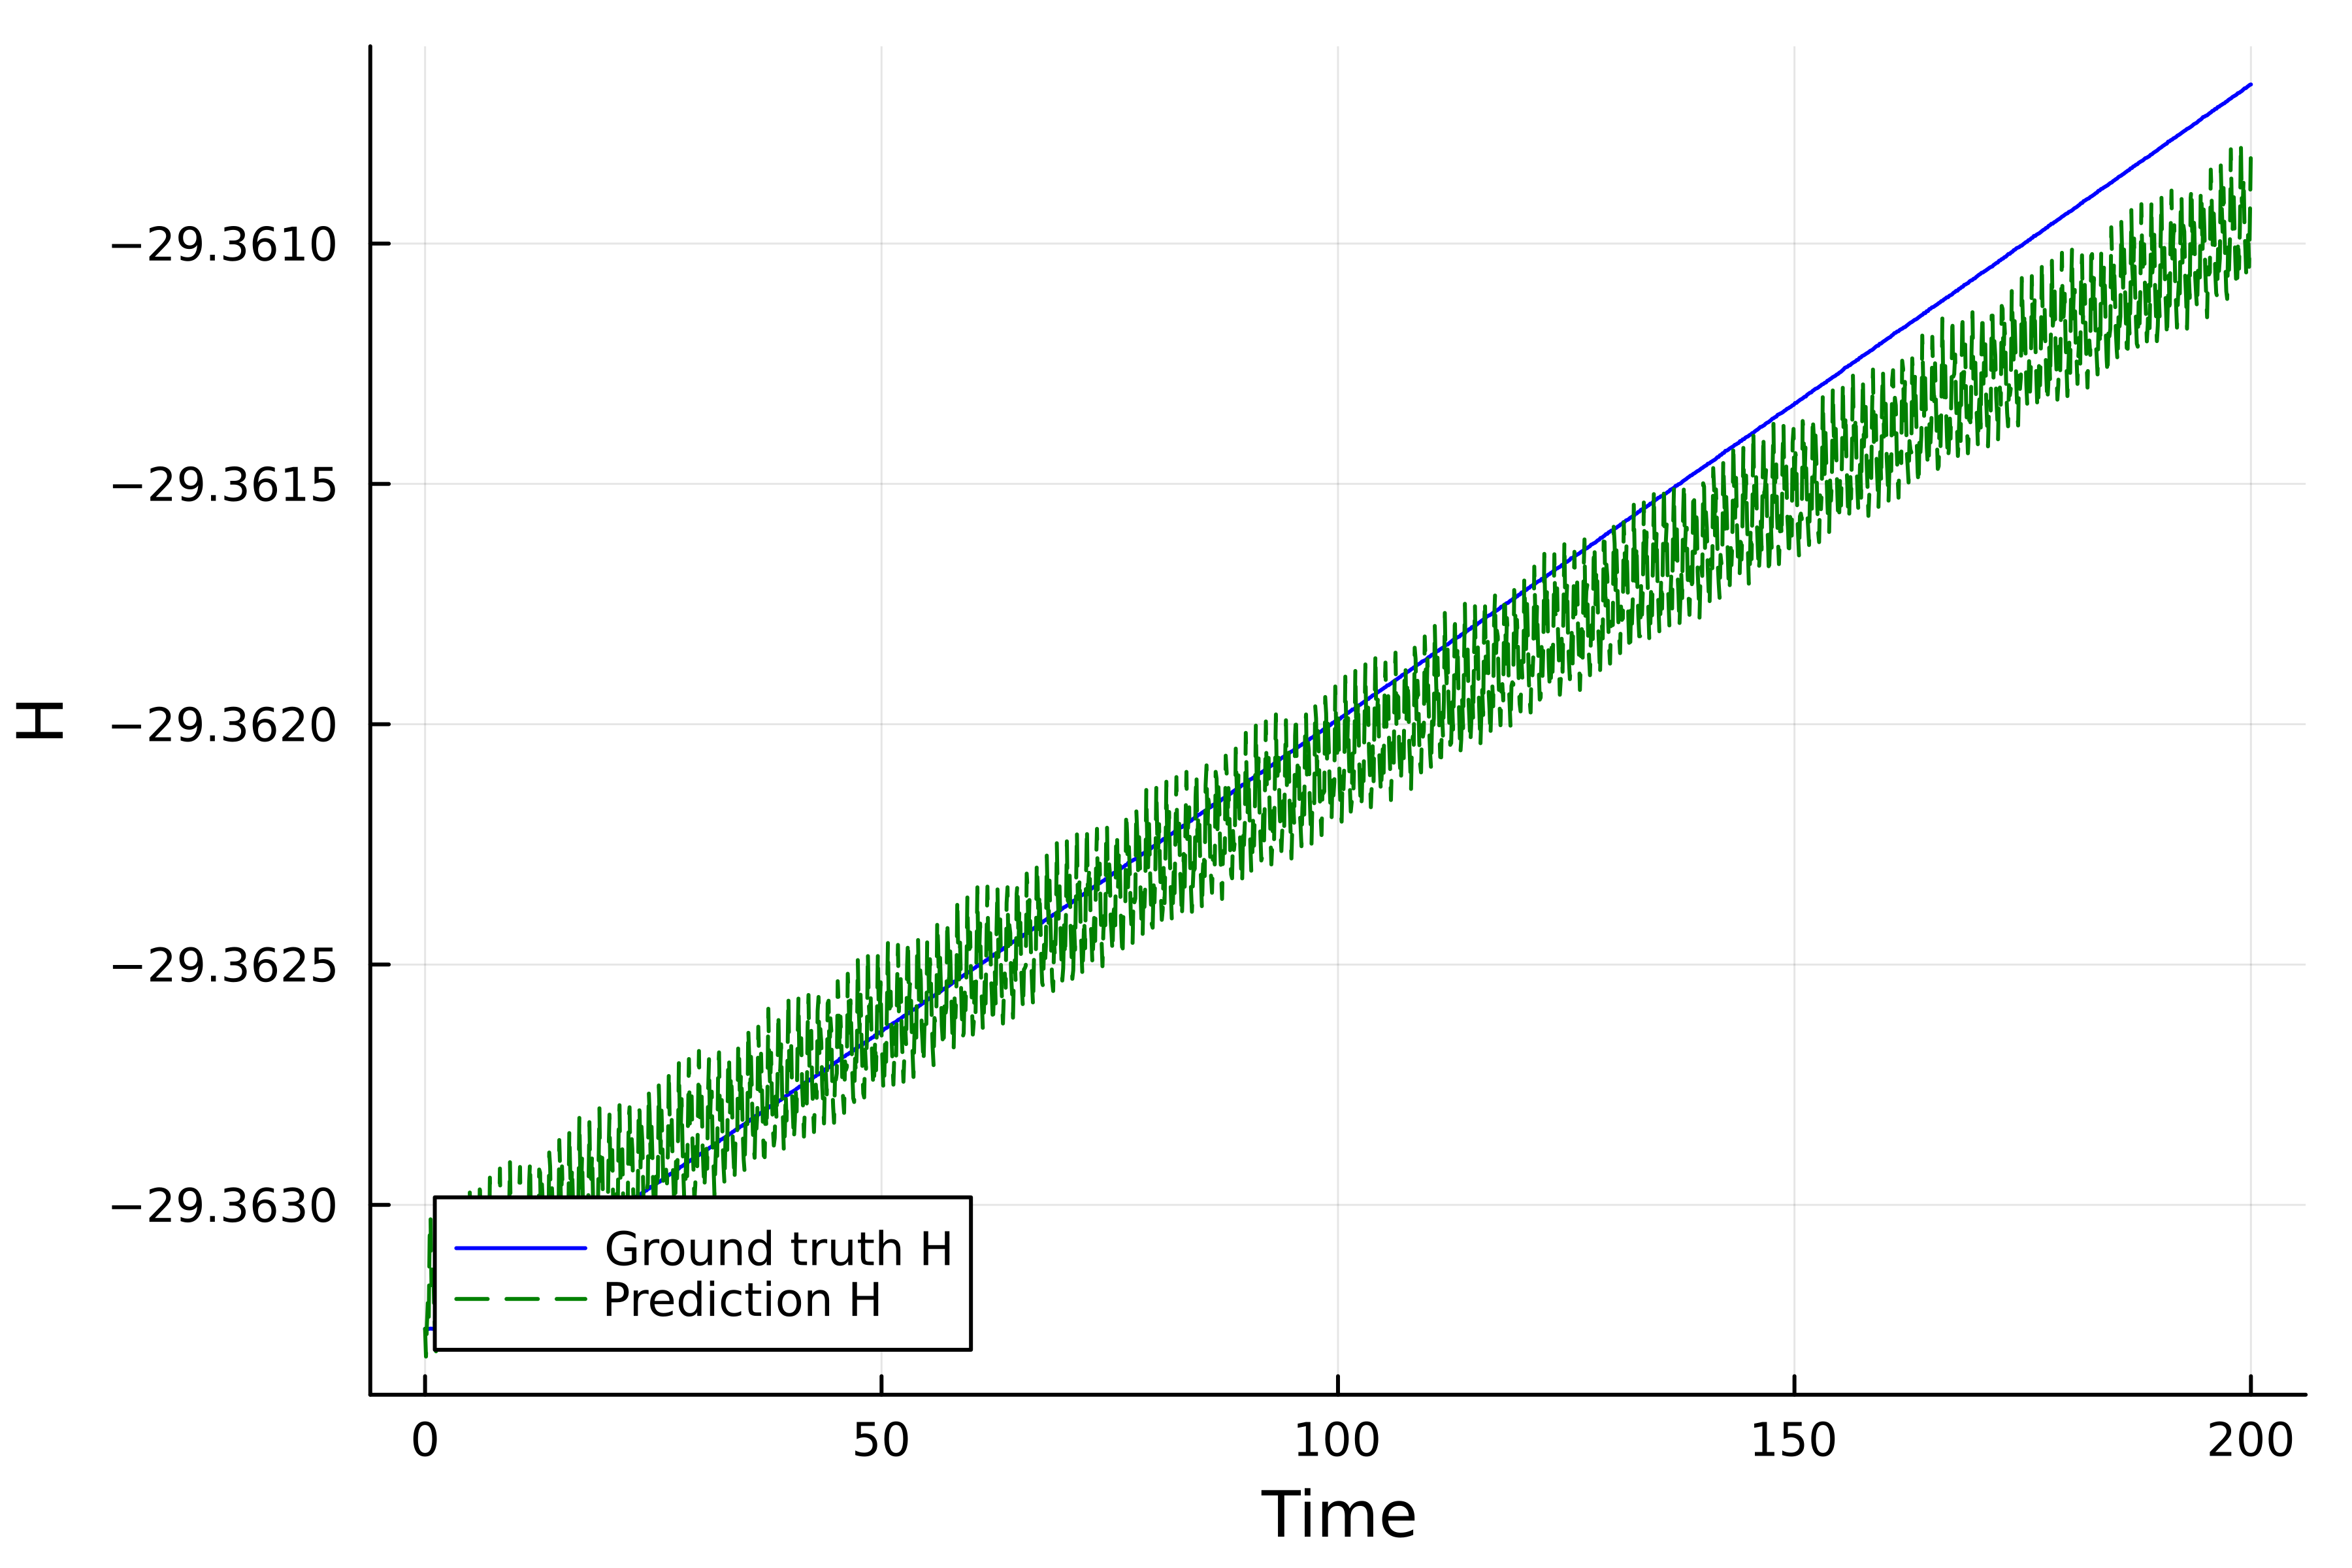
\includegraphics[width=0.5\linewidth]{../examples/double_pendulum_hnn/hamiltonian}
	\caption{Example \ref{ex:hnn_double_pendulum}. Hamiltonian of ODE and HNN solutions outside the training interval.}
	\label{fig:hnn_double_pendulum_hamiltonian}
\end{figure}

\bibliographystyle{siamplain}
\bibliography{references}

\end{document}
